\documentclass{article}
\usepackage{booktabs}
\usepackage{amsmath}
\usepackage{graphicx}
\usepackage{fullpage}
\usepackage[utf8]{inputenc}
\usepackage[T1]{fontenc}
\usepackage{amsfonts}
\usepackage[spanish]{babel}
\usepackage{xcolor}
\usepackage{float}
\usepackage{subcaption}
\usepackage{hyperref}
\usepackage{amssymb}
\hypersetup{
    colorlinks=true,       % False para cuadros, true para texto coloreado
    linkcolor=black,        % Color para enlaces internos (índice)
    urlcolor=blue,         % Color para URLs externas
    pdftitle={Mi Documento} % Metadatos del PDF
}

% Datos del documento
\newcommand{\eltitulo}{Predicción del riesgo de\\ adicción a los videojuegos}
\newcommand{\elautor}{Pablo Carro Arcaya, Miguel Pérez Ciriaco}
\newcommand{\lafecha}{\today}

\begin{document}

% ---------------- PORTADA ----------------
\begin{titlepage}
    \centering

    \vspace*{\fill}
    
    \vspace{1cm}
    \vspace{1.5cm}

    {\Huge\bfseries \eltitulo \par}
    
    \vspace{1cm}

    \vspace{2cm}

        {\Large
    \textsc{Minería de datos}\par}
    \vspace{1cm}

    {\large
    \elautor\par}

    \vspace{2cm}

    {\large \lafecha \par}

    \vspace*{\fill}

\end{titlepage}
% ----------------------------------------

\tableofcontents
\pagebreak

\section{Introducción}

En cualquier problema de aprendizaje automático a resolver, la calidad de las soluciones obtenidas depende en gran medida de la calidad de la información disponible.
Existen multitud de técnicas que permiten aumentar la calidad de un dataset, ya sea limpiándolo de ejemplos con ruido o modificando el contenido
de las variables para que, sin perder información sobre el problema, los modelos mejoren su rendimiento.\newline

En este proyecto se pretende hacer uso de las principales técnicas de minería de datos para resolver un problema de clasificación binaria no balanceado.

\subsection{El problema}

El problema elegido consiste en medir el nivel de riesgo de adicción a los videojuegos, clasificando a los individuos en dos grupos: personas con riesgo \textit{bajo} (en adelante clase 0),
y personas con riesgo \textit{alto} (en adelante clase 1). Para ello, se ha empleado el dataset \textit{\href{https://www.kaggle.com/datasets/shaistashahid/gaming-and-mental-health}{Gaming and Mental Health}}, que contiene datos sobre la salud mental y física de diferentes individuos, así como información sobre el día a día de los mismos, todo ello junto a una etiqueta que indica su nivel de riesgo\footnote{En el dataset original existen 4 niveles de riesgo. Para transformar el problema a clasificación binaria, se han agrupado los dos mas bajos, y los dos más altos}.\newline

La propoción de individuos de ambas clases dentro del dataset es de un 70-30, siendo el grupo de riesgo \textit{bajo} la clase mayoritaria y el de riesgo \textit{alto} la minoritaria. Este dataset comprende una amplia variedad de aspectos sobre cada individuo. Contiene tanto variables categóricas como la calidad del sueño o el estado de ánimo general, como variables numéricas, como el tiempo de juego diario o el dinero invertido al mes en videojuegos.\newline

comentar que el dataset es sintético

ver si poner algo más. no estoy muy convencido. estaba pensando en explicar aquí que interesa no fallar los individuos de riesgo alto

\subsection{Relación de las variables de entrada con la variable de salida}

Para obtener una primera impresión sobre el comportamiento de cada variable según la clase, se han elaborado las siguientes gráficas:

\subsubsection{Variables numéricas}

\begin{figure}[H]
    \centering
    \begin{subfigure}[b]{0.48\textwidth}
        \centering
        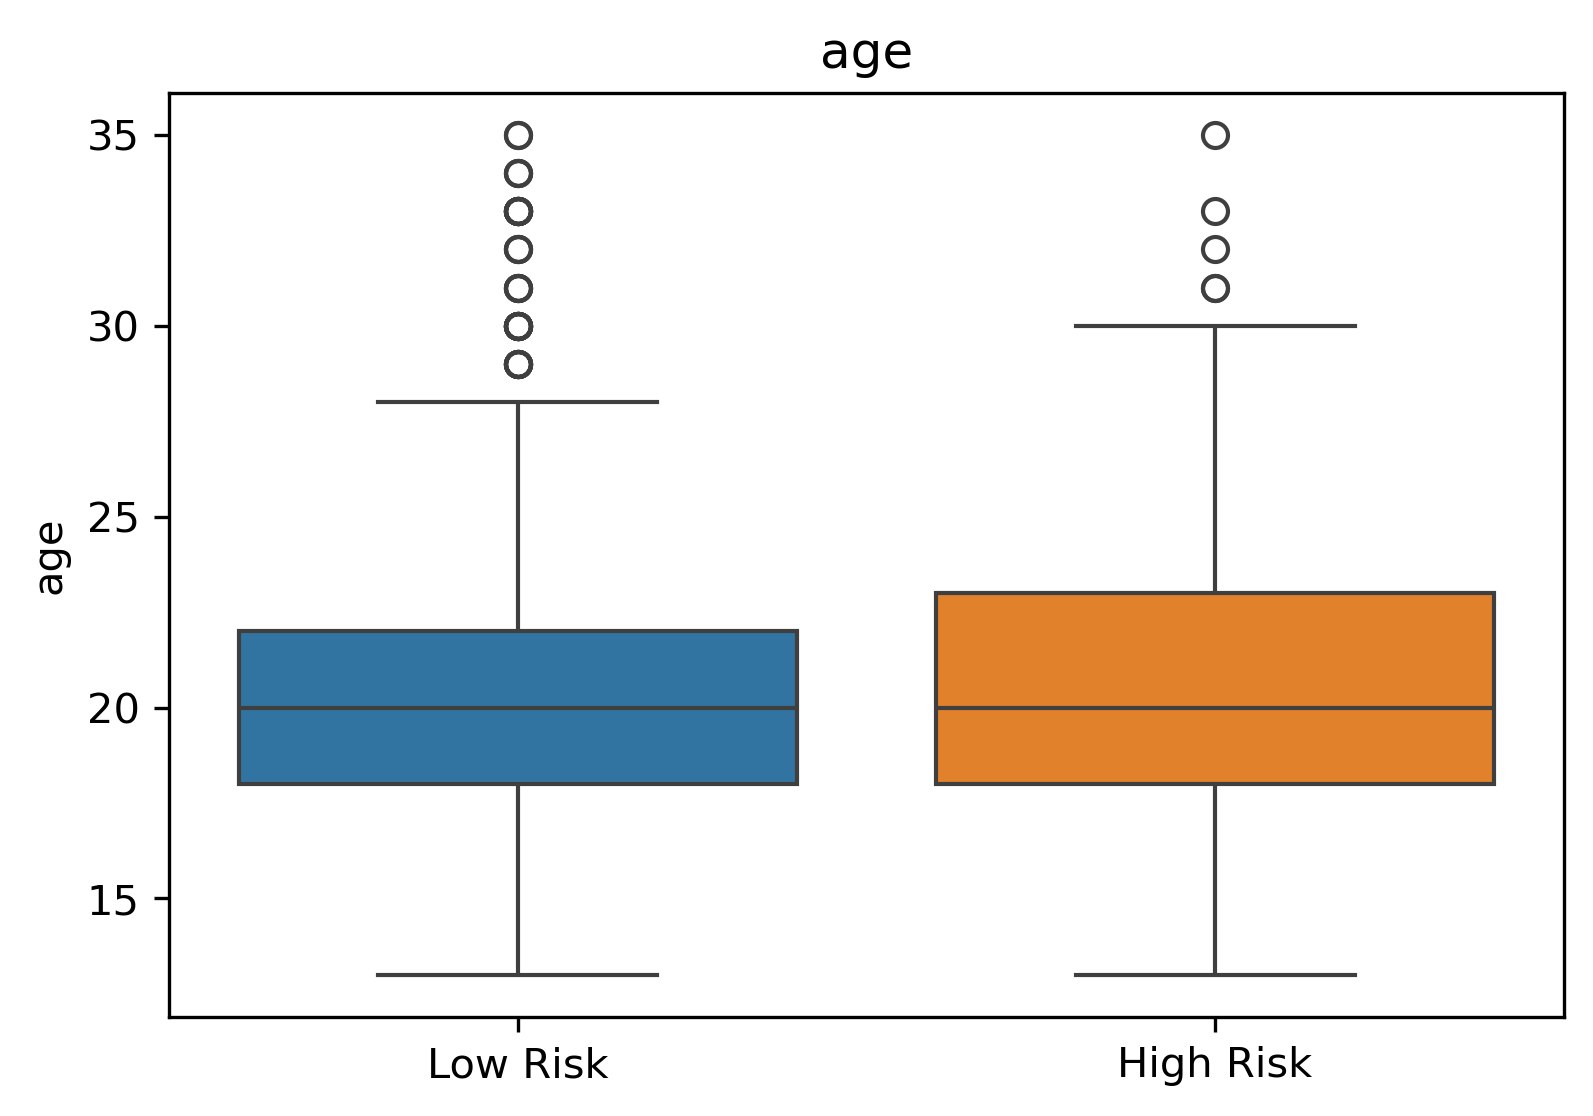
\includegraphics[width=\textwidth]{images/numericas/age.png}
        \caption{Distribución de Edad}

    \end{subfigure}
    \hfill
    \begin{subfigure}[b]{0.48\textwidth}
        \centering
        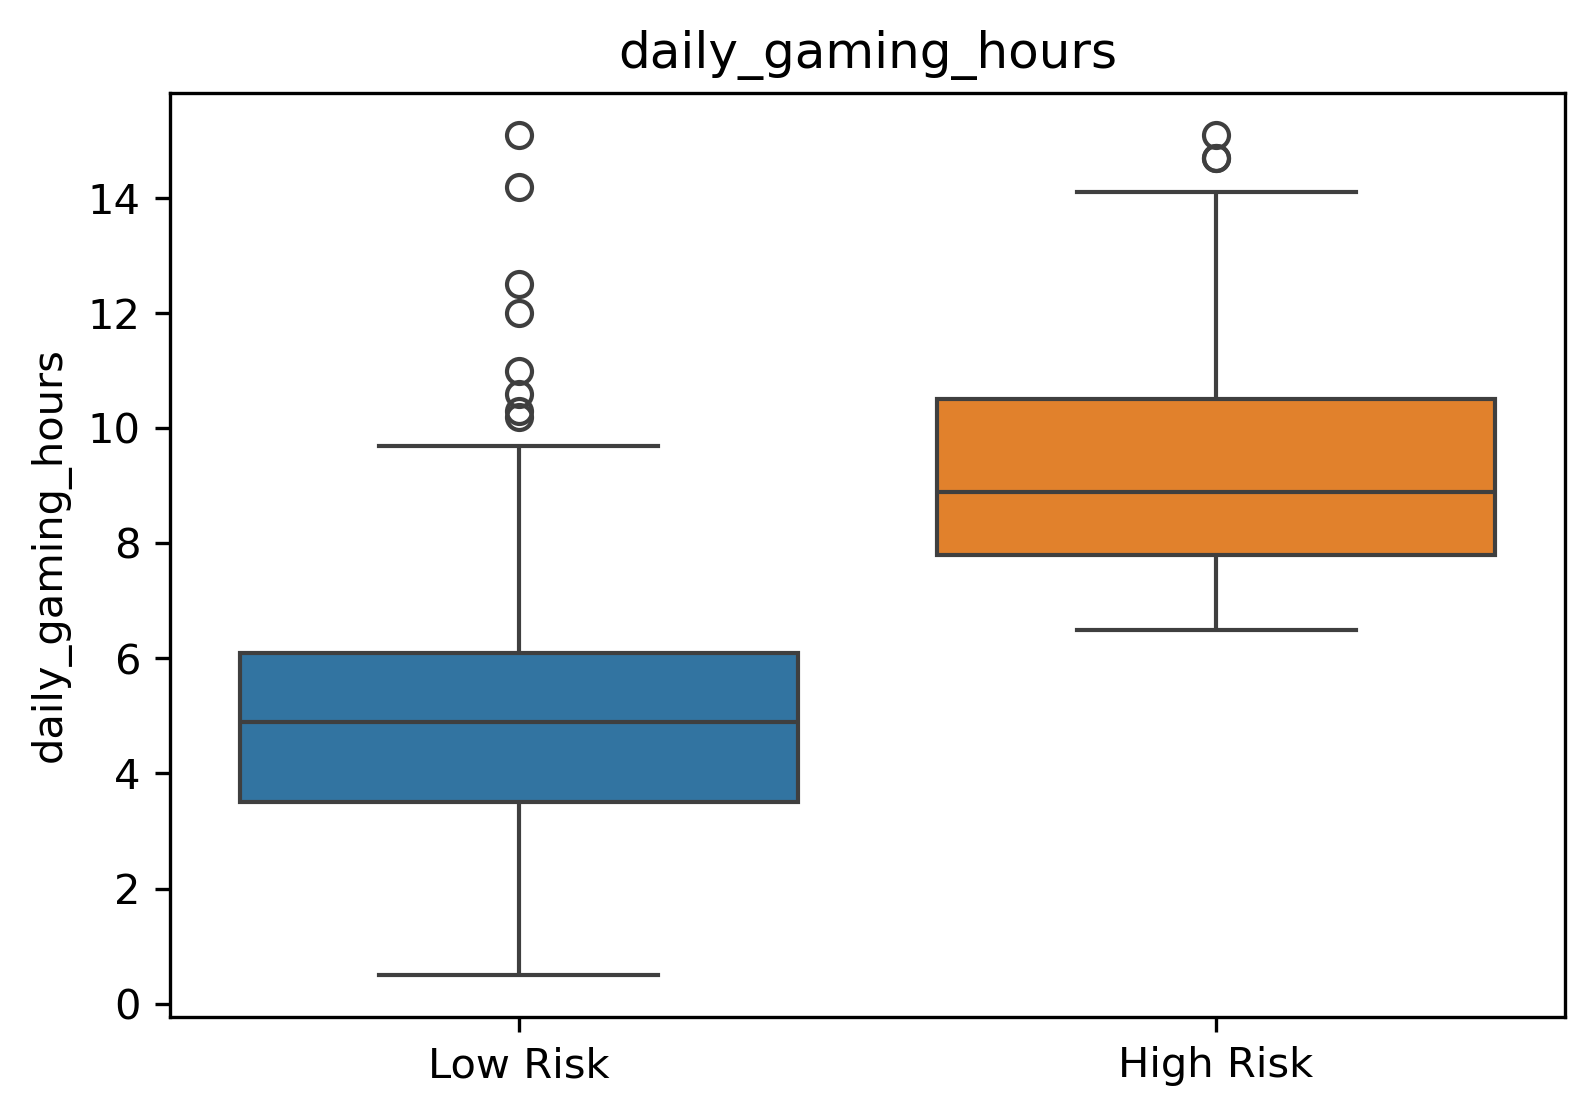
\includegraphics[width=\textwidth]{images/numericas/daily_gaming_hours.png}
        \caption{Horas de juego semanales}

    \end{subfigure}

    \vspace{10pt}

\end{figure}
\begin{figure}[H]
    \centering
    \ContinuedFloat % Para que el contador de la figura no salte si quieres mantener el mismo número
    \begin{subfigure}[b]{0.48\textwidth}
        \centering
        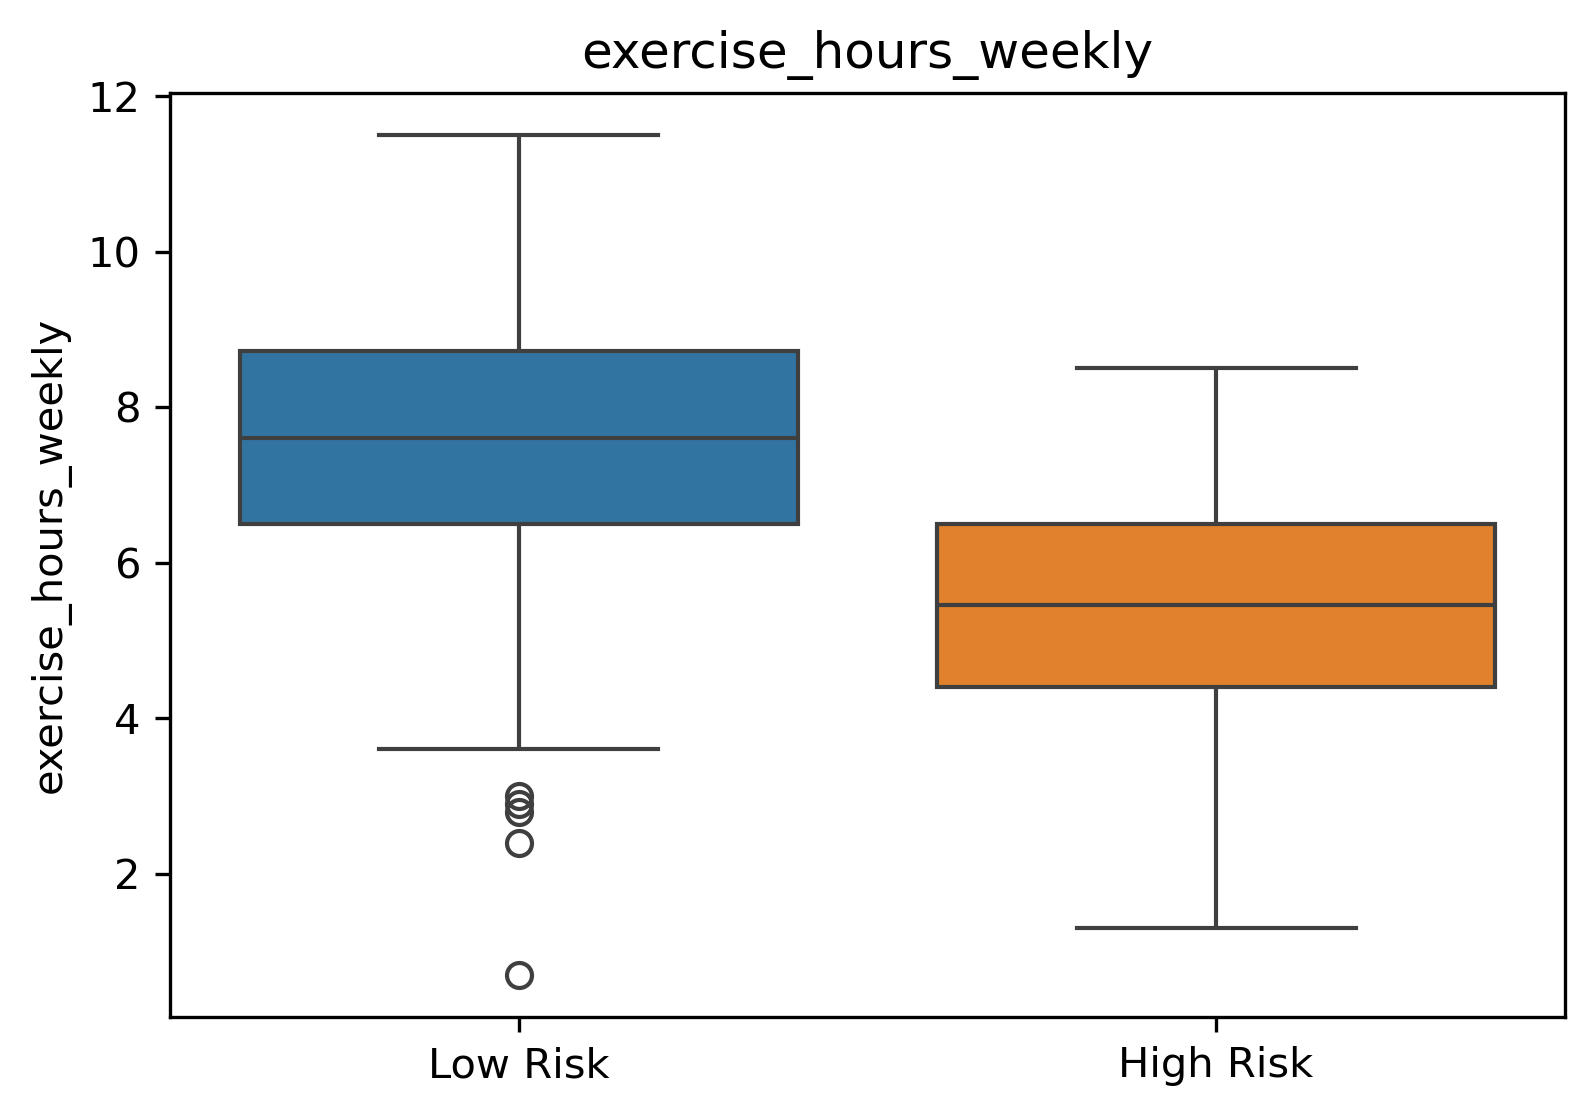
\includegraphics[width=\textwidth]{images/numericas/exercise_hours_weekly.png}
        \caption{Horas de ejercicio semanal}

    \end{subfigure}
    \hfill % Esto añade espacio elástico entre las dos imágenes
    \begin{subfigure}[b]{0.48\textwidth}
        \centering
        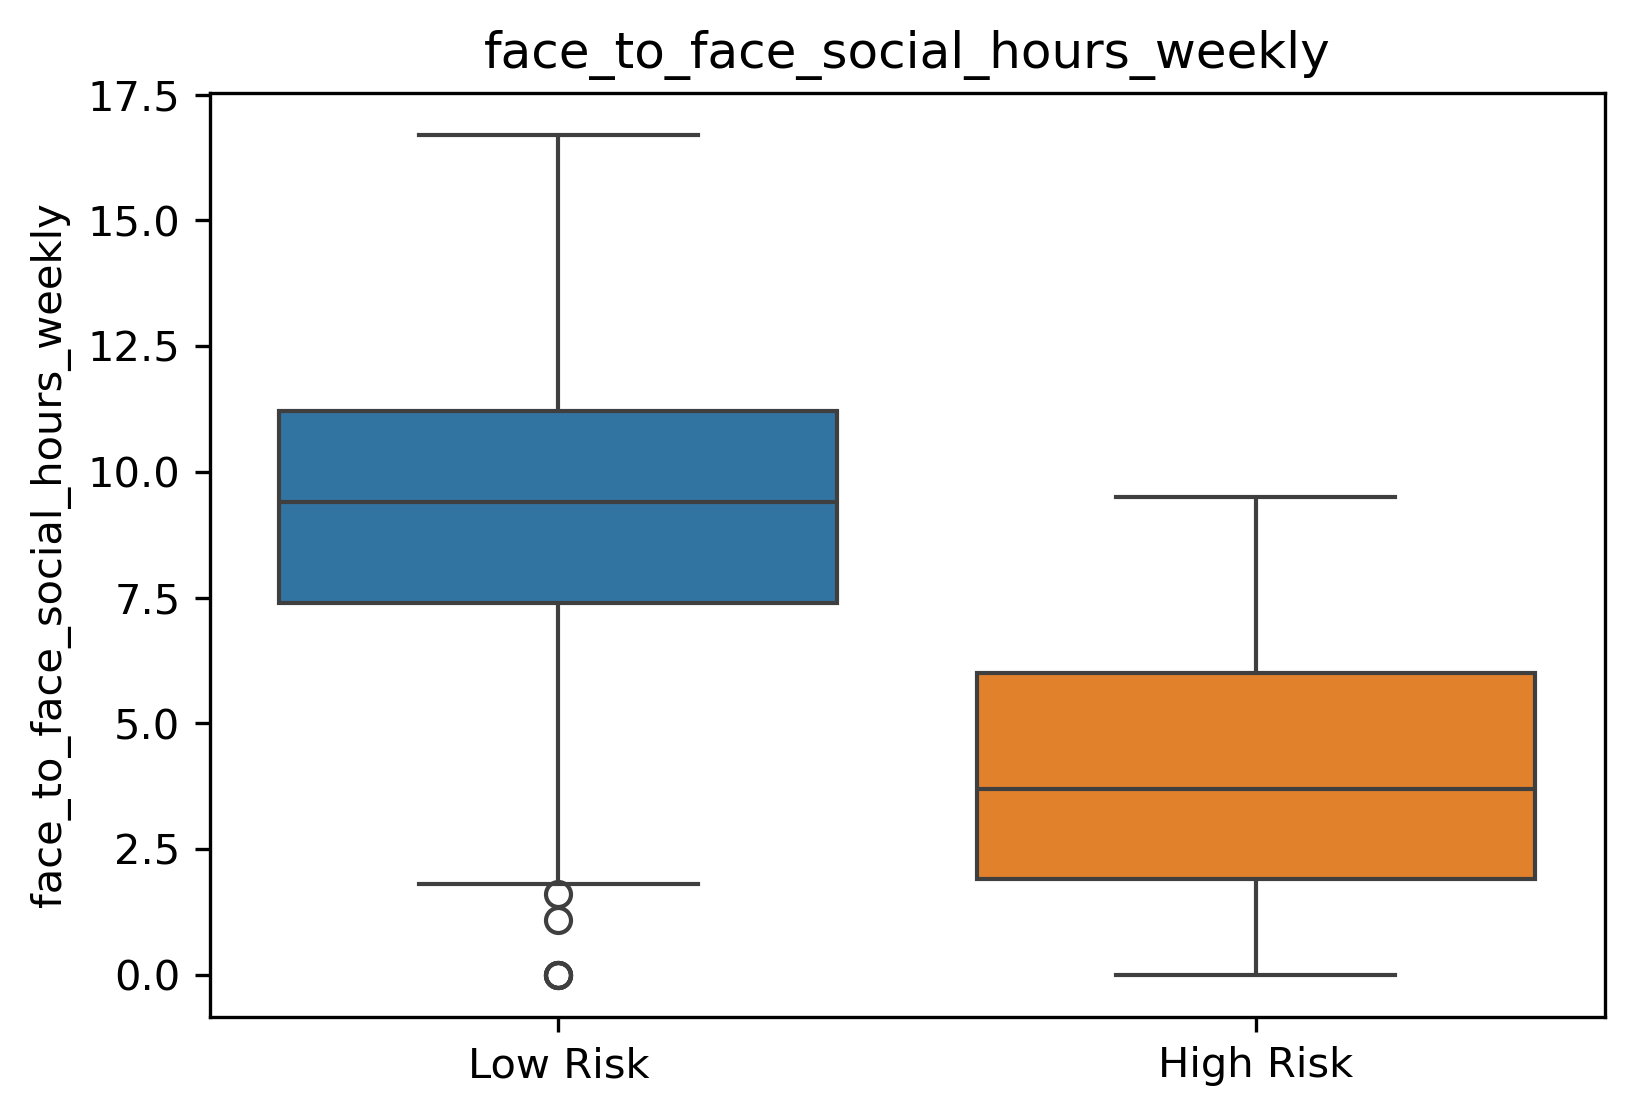
\includegraphics[width=\textwidth]{images/numericas/face_to_face_social_hours_weekly.png}
        \caption{Horas de socialización en persona semanales}

    \end{subfigure}

    \vspace{10pt}

    \begin{subfigure}[b]{0.48\textwidth}
        \centering
        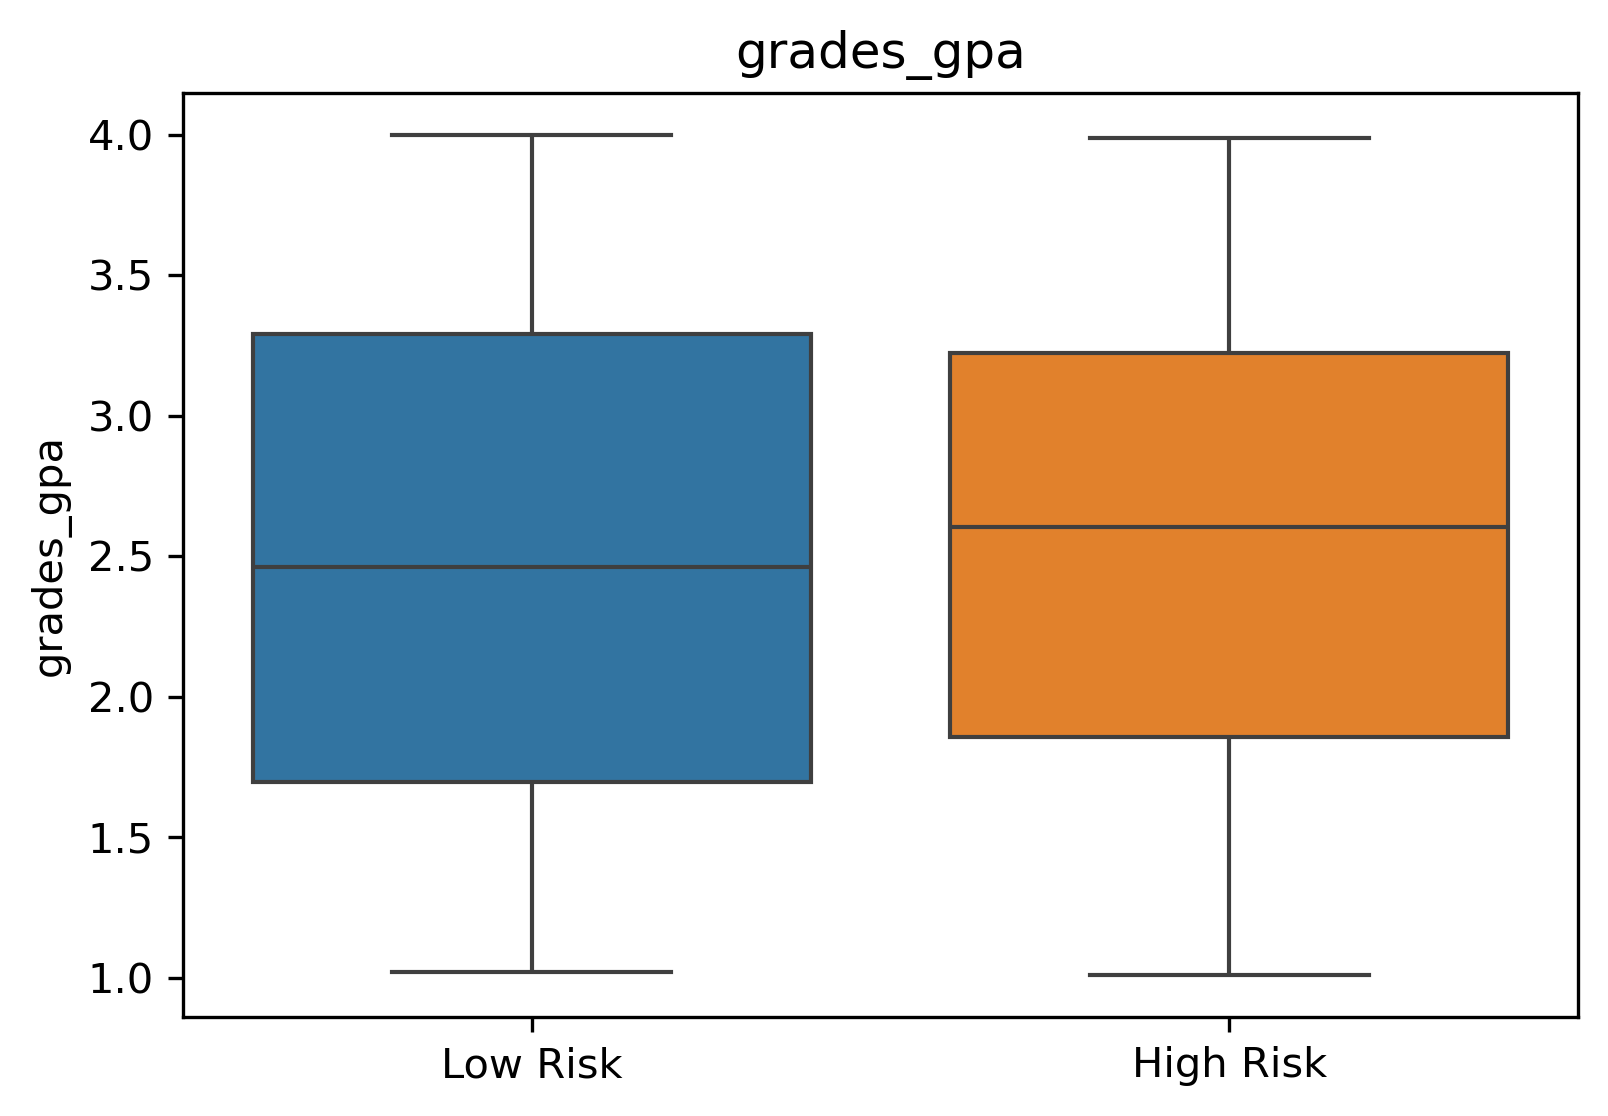
\includegraphics[width=\textwidth]{images/numericas/grades_gpa.png}
        \caption{Nota media}

    \end{subfigure}
    \hfill % Esto añade espacio elástico entre las dos imágenes
    \begin{subfigure}[b]{0.48\textwidth}
        \centering
        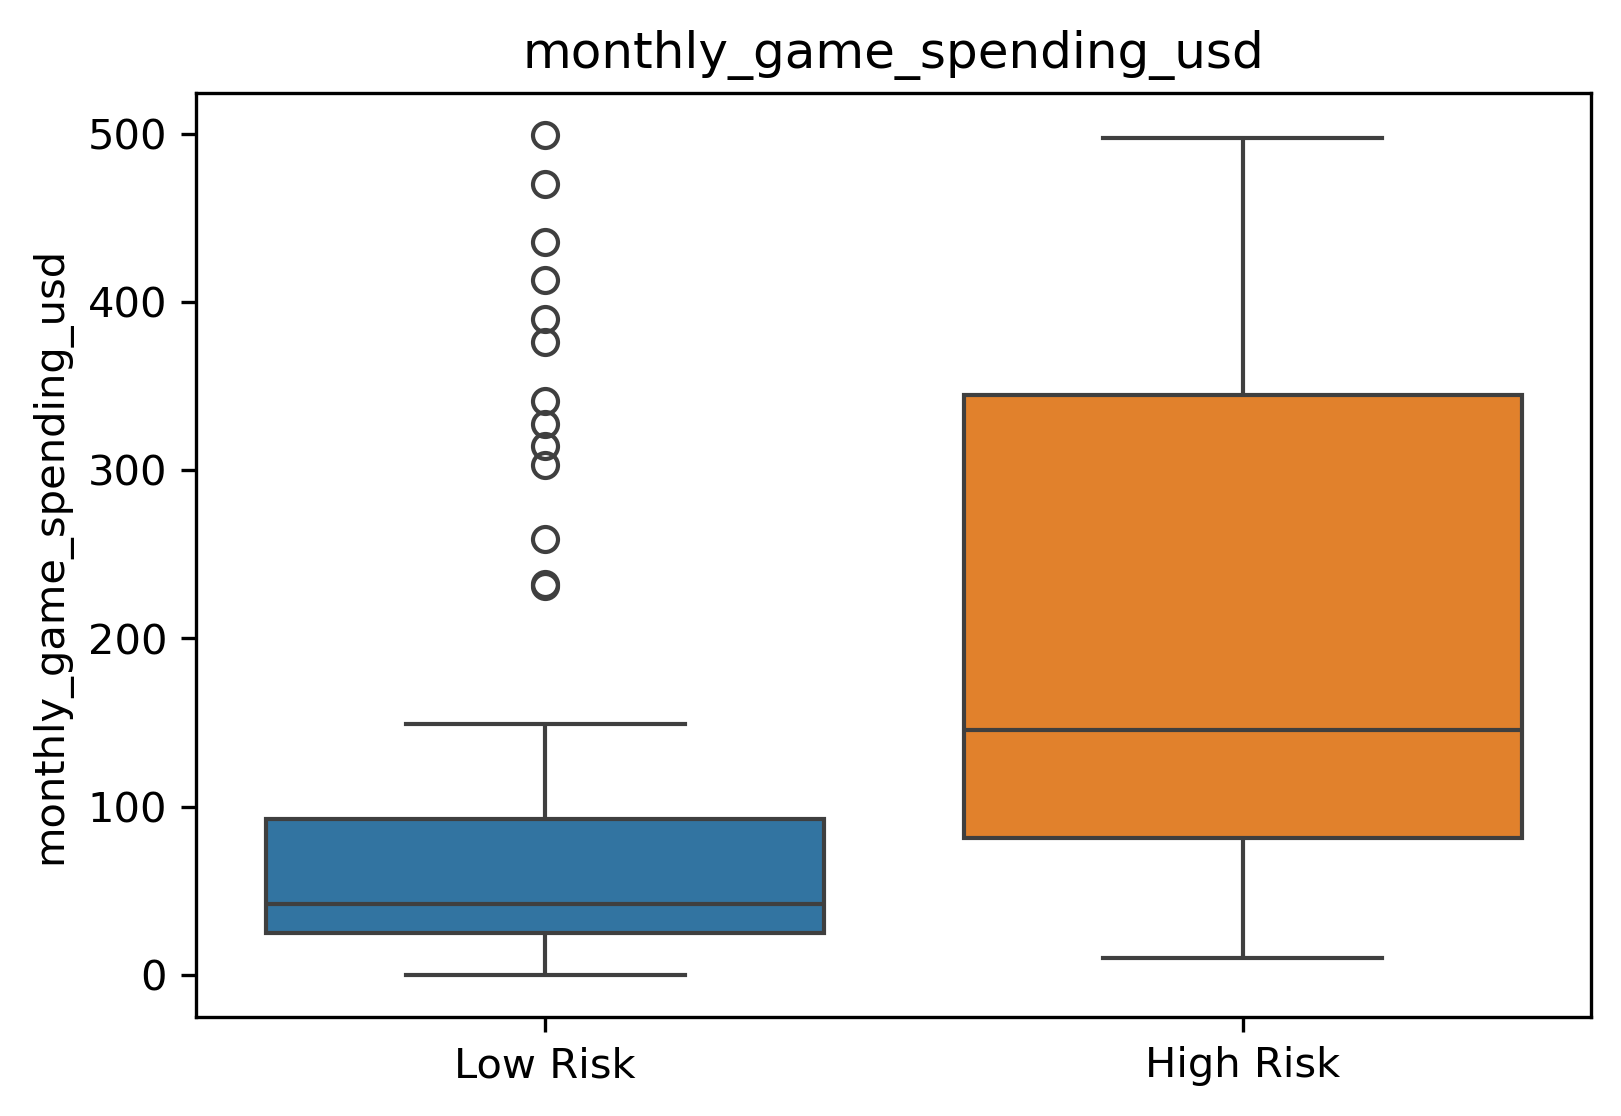
\includegraphics[width=\textwidth]{images/numericas/monthly_game_spending_usd.png}
        \caption{Gasto mensual en videojuegos}

    \end{subfigure}

    \vspace{10pt}

    \begin{subfigure}[b]{0.48\textwidth}
        \centering
        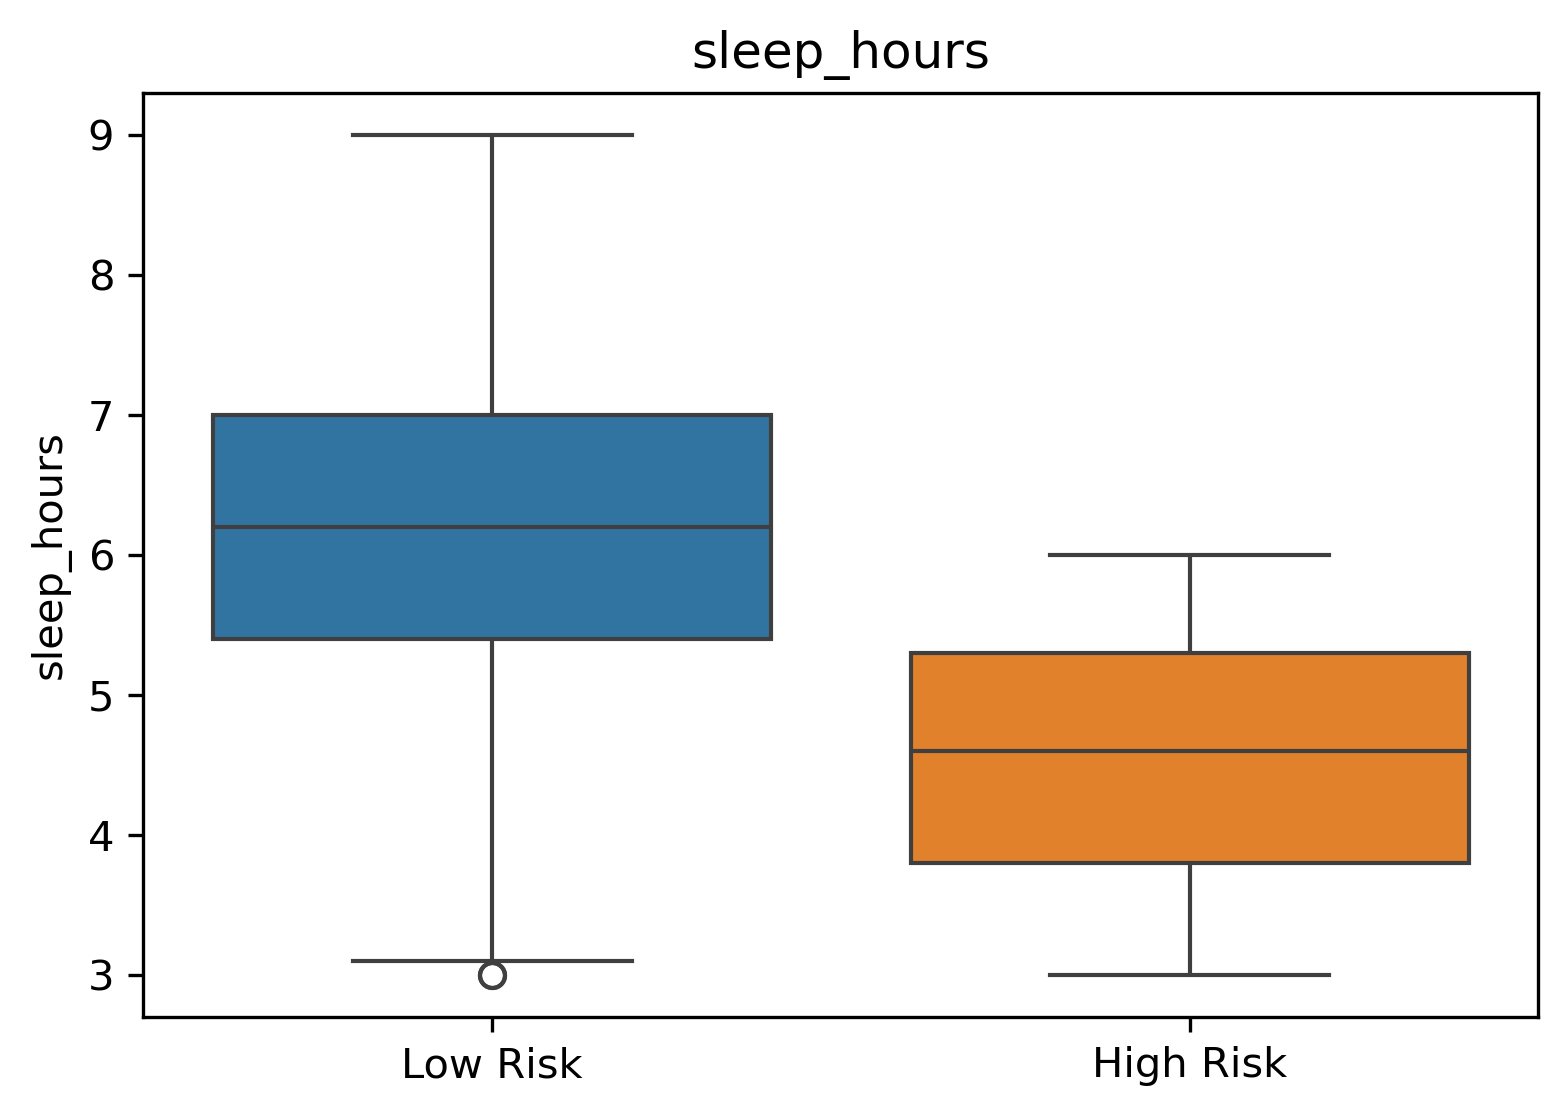
\includegraphics[width=\textwidth]{images/numericas/sleep_hours.png}
        \caption{Horas de sueño diarias}

    \end{subfigure}
    \hfill % Esto añade espacio elástico entre las dos imágenes
    \begin{subfigure}[b]{0.48\textwidth}
        \centering
        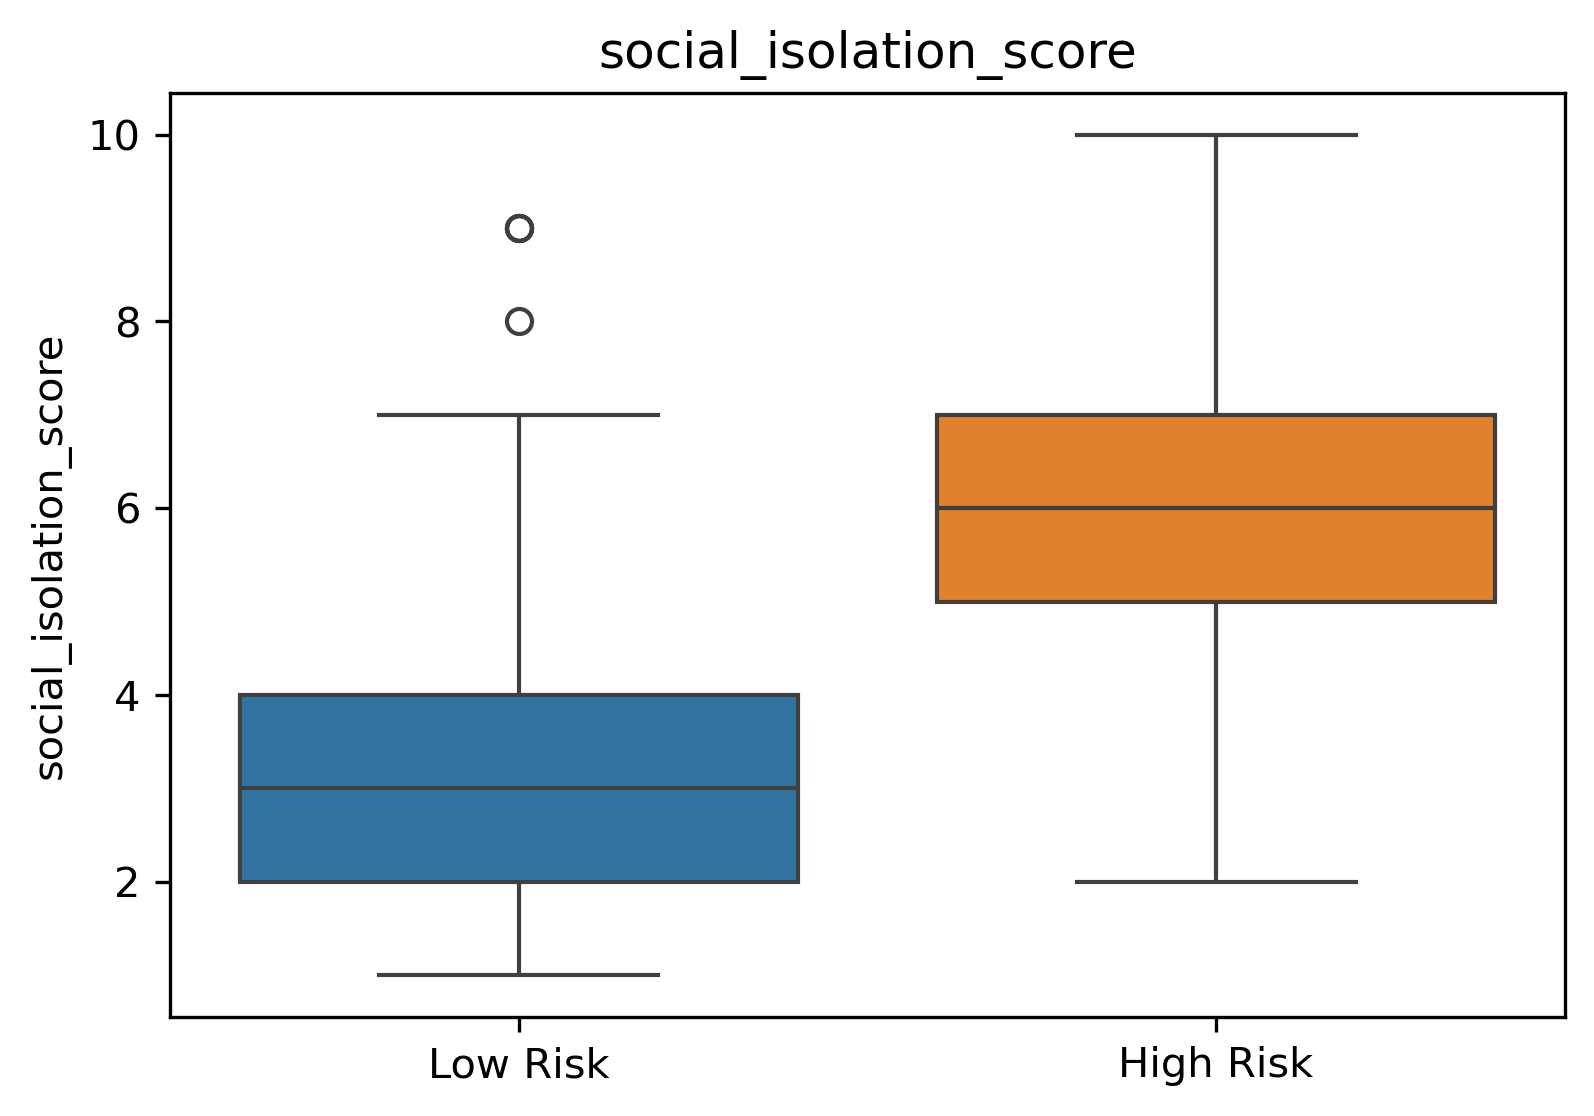
\includegraphics[width=\textwidth]{images/numericas/social_isolation_score.png}
        \caption{Nivel de aislamiento social}

    \end{subfigure}

    \vspace{10pt}

\end{figure}
\begin{figure}[H]
    \centering
    \ContinuedFloat % Para que el contador de la figura no salte si quieres mantener el mismo número
    \begin{subfigure}[b]{0.48\textwidth}
        \centering
        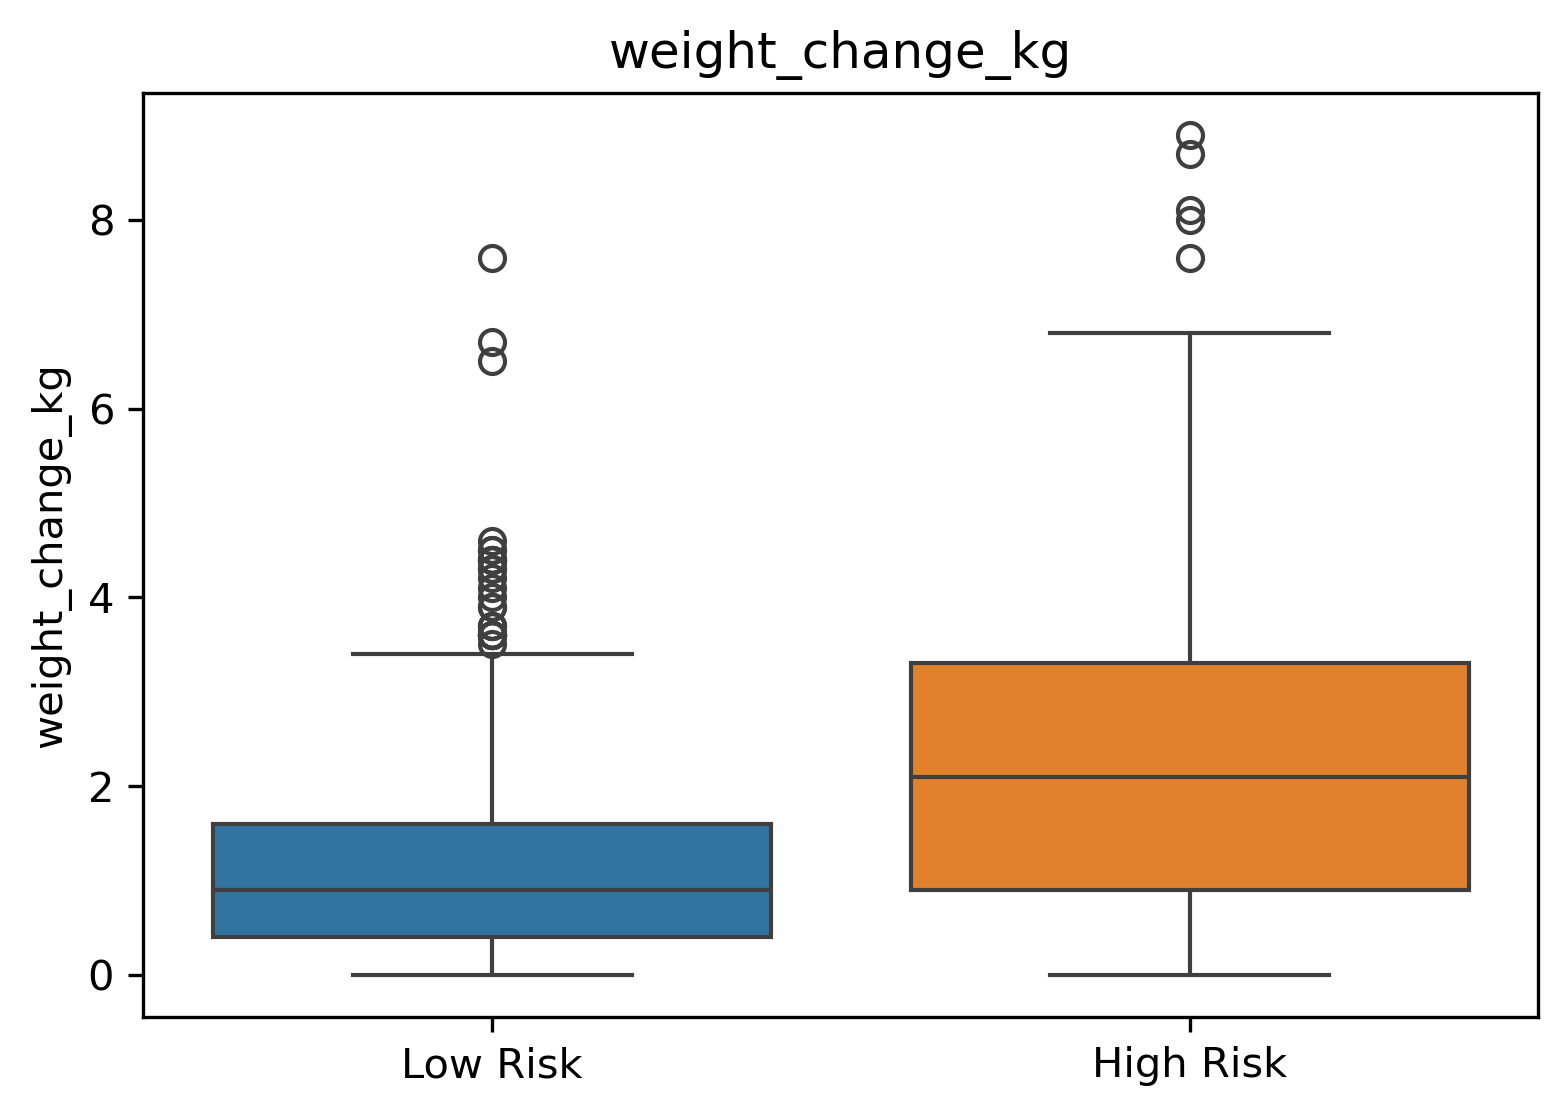
\includegraphics[width=\textwidth]{images/numericas/weight_change_kg.png}
        \caption{Ganancia de peso}

    \end{subfigure}
    \hfill % Esto añade espacio elástico entre las dos imágenes
    \begin{subfigure}[b]{0.48\textwidth}
        \centering
        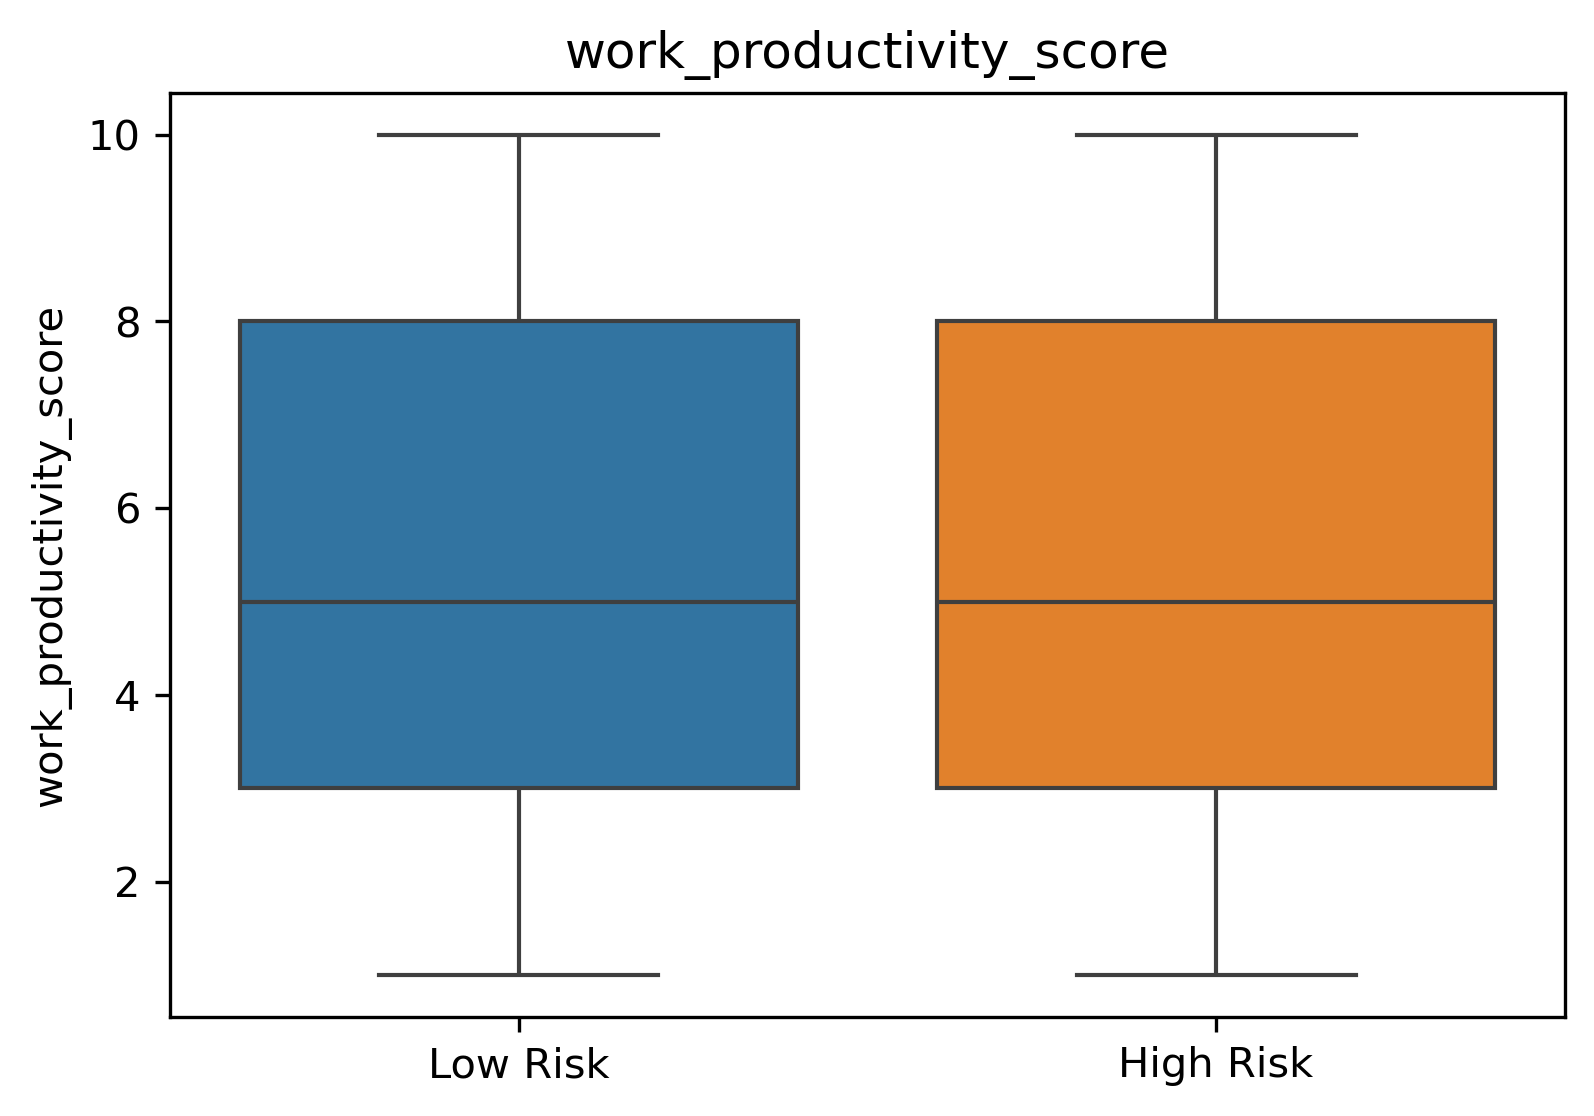
\includegraphics[width=\textwidth]{images/numericas/work_productivity_score.png}
        \caption{Nivel de productividad en el trabajo}

    \end{subfigure}

    \vspace{10pt}

    \begin{subfigure}[b]{0.48\textwidth}
        \centering
        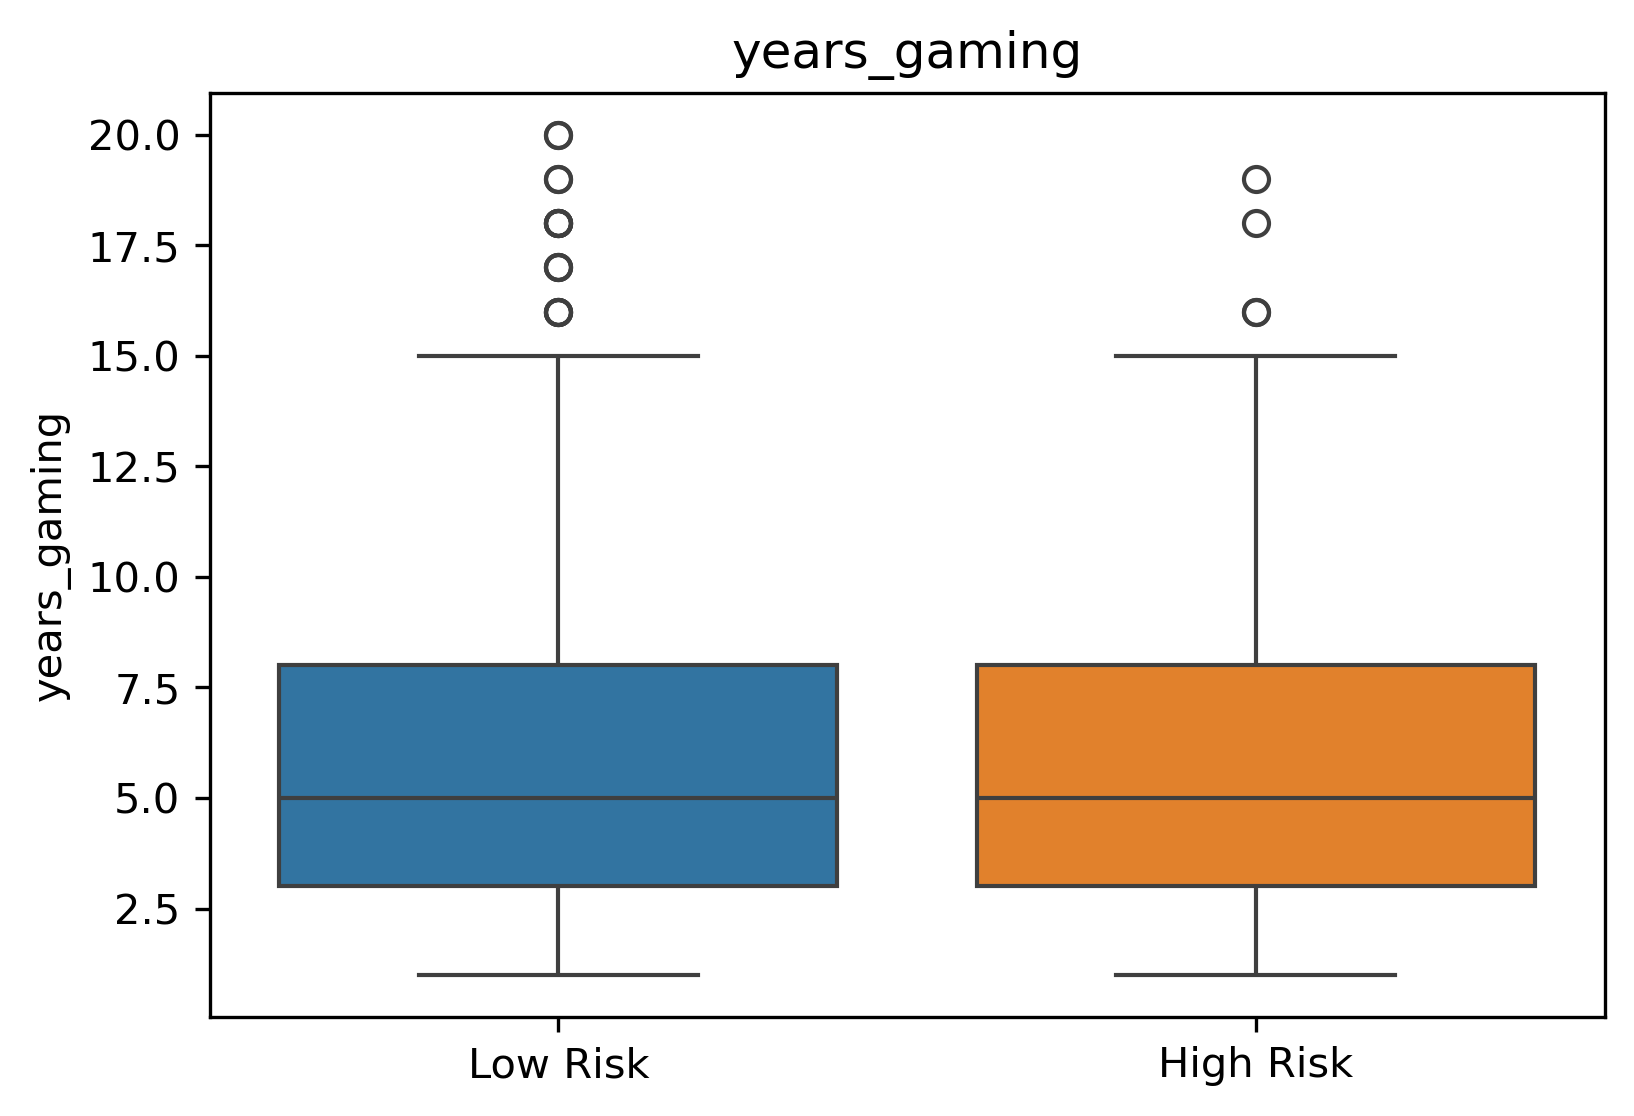
\includegraphics[width=\textwidth]{images/numericas/years_gaming.png}
        \caption{Años jugando videojuegos}

    \end{subfigure}

    \caption{Diagramas de caja y bigotes de cada variable numérica según la clase.}
    \label{fig:analisis_numerico}
\end{figure}

En las gráficas se aprecia que algunas variables se comportan de manera muy similar independientemente de la clase a la que pertenezcan. Ejemplos de ello son las variables: \textit{edad}, \textit{GPA} (nota media), \textit{years\_gaming} o \textit{work\_productivity\_score}.\newline

Sin embargo, existen variables que cambian de manera muy marcada según la clase. Por ejemplo, se observa que los individuos con alto riesgo de adicción son los que menos socializan en persona
(\textit{face\_to\_face\_social\_hours}, \textit{social\_isolation\_score}), los que menos ejercicio hacen (\textit{exercise\_hours}) y los que menos duermen (\textit{sleep\_hours}). \newline

Además, los gastos en juegos son mayores en personas con alto riesgo (\textit{monthly\_game\_spending\_usd}), así como la ganancia de peso (\textit{weight\_change\_kg}) y, naturalmente, las horas de juego diarias (\textit{daily\_gaming\_hours}).

\newpage
\subsubsection{Variables categóricas (por clase)}
\begin{figure}[H]
    \centering
    \begin{subfigure}[b]{0.48\textwidth}
        \centering
        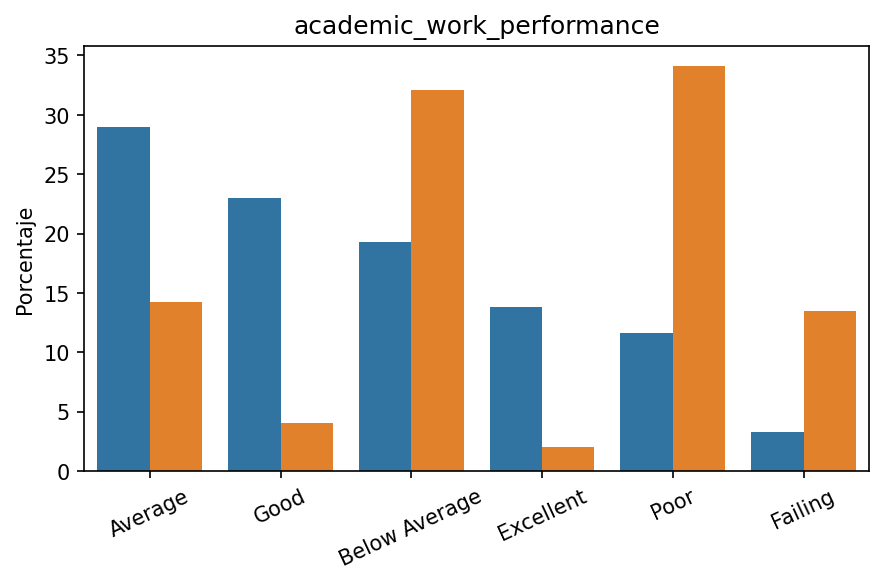
\includegraphics[width=\textwidth]{images/categoricas/academic_work_performance.png}
        \caption{Rendimiento académico/laboral}
    \end{subfigure}
    \hfill
    \begin{subfigure}[b]{0.48\textwidth}
        \centering
        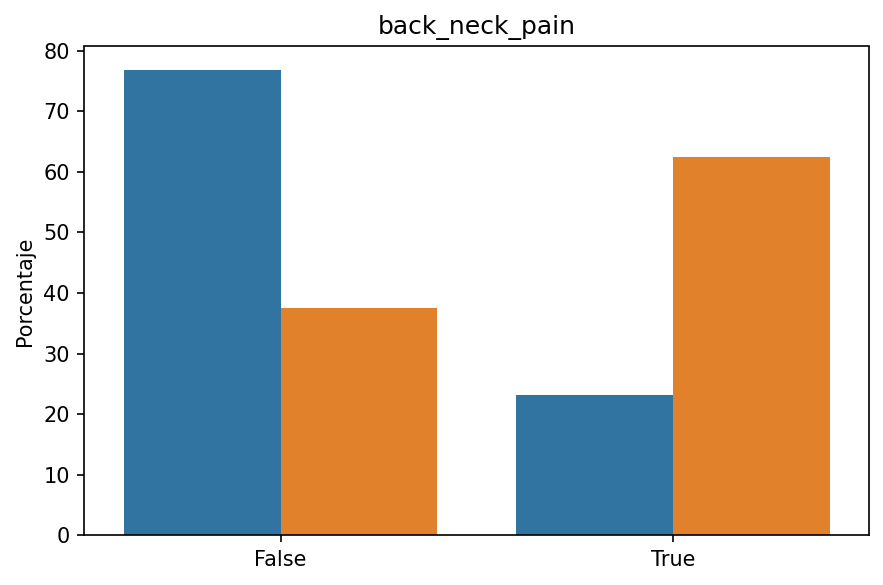
\includegraphics[width=\textwidth]{images/categoricas/back_neck_pain.png}
        \caption{Dolor de espalda/cuello}
    \end{subfigure}
    \vspace{10pt}
    \begin{subfigure}[b]{0.48\textwidth}
        \centering
        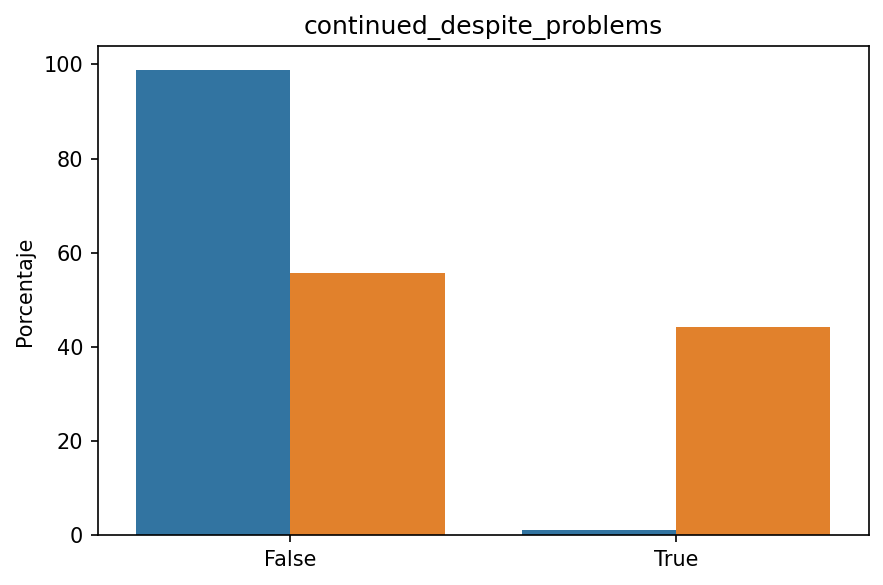
\includegraphics[width=\textwidth]{images/categoricas/continued_despite_problems.png}
        \caption{Continúa jugando a pesar de los problemas}
    \end{subfigure}
    \hfill
    \begin{subfigure}[b]{0.48\textwidth}
        \centering
        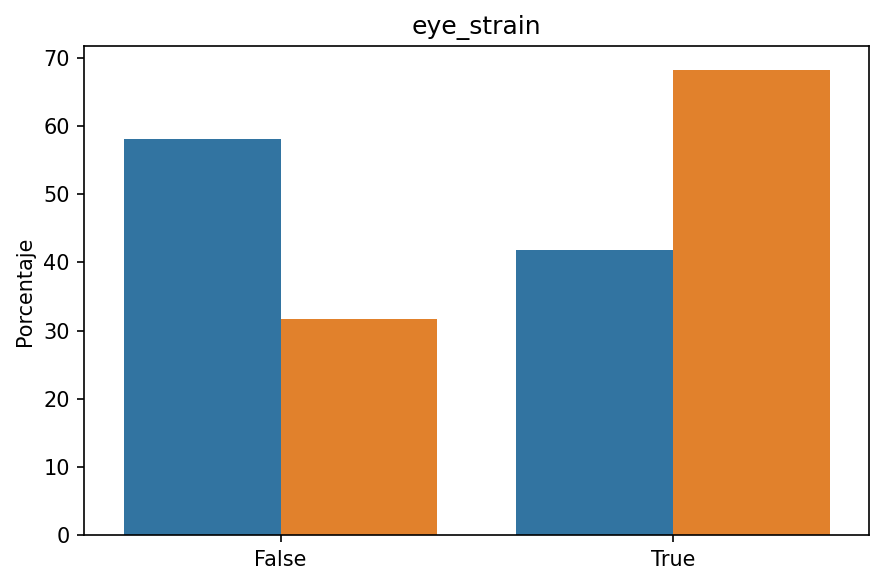
\includegraphics[width=\textwidth]{images/categoricas/eye_strain.png}
        \caption{Fatiga visual}
    \end{subfigure}
    \vspace{10pt}
    \begin{subfigure}[b]{0.48\textwidth}
        \centering
        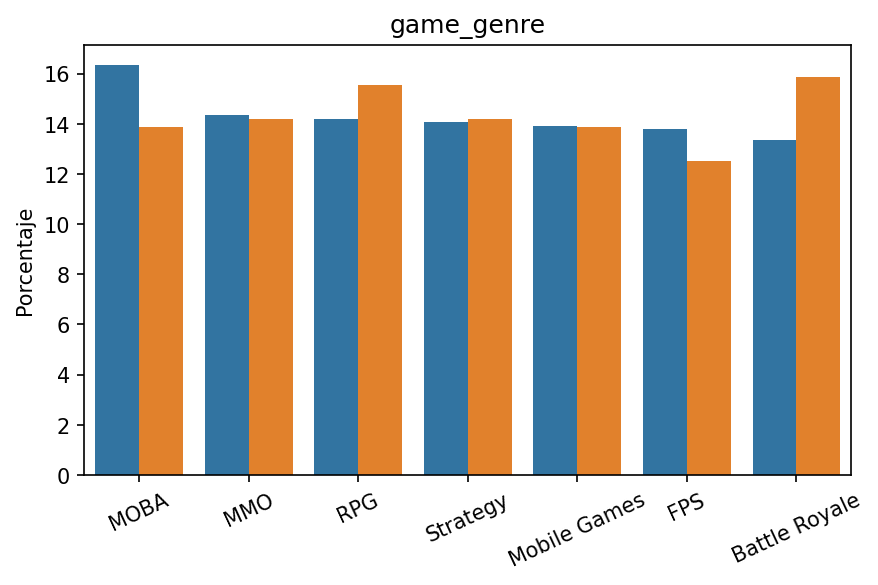
\includegraphics[width=\textwidth]{images/categoricas/game_genre.png}
        \caption{Género de videojuego}
    \end{subfigure}
    \hfill
    \begin{subfigure}[b]{0.48\textwidth}
        \centering
        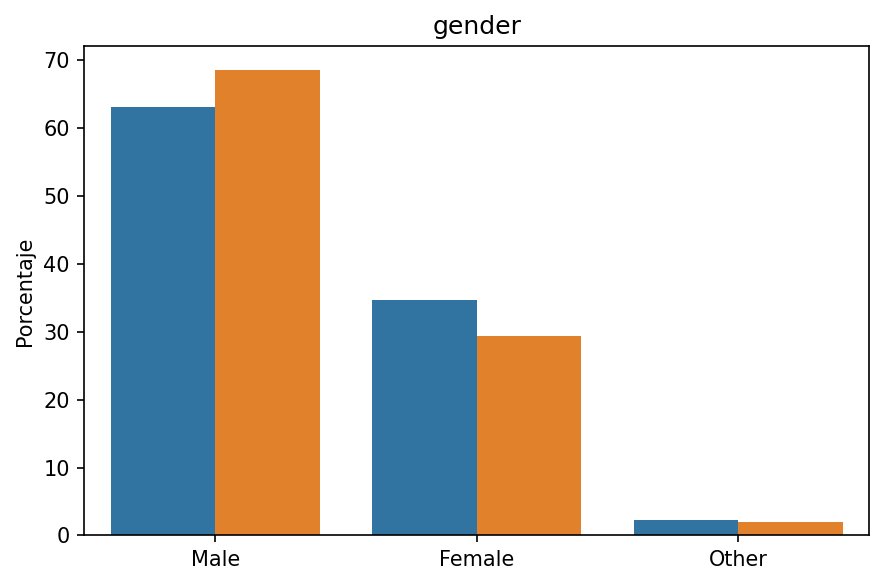
\includegraphics[width=\textwidth]{images/categoricas/gender.png}
        \caption{Género}
    \end{subfigure}
    \vspace{10pt}
\end{figure}
\begin{figure}[H]
    \centering
    \ContinuedFloat
    \begin{subfigure}[b]{0.48\textwidth}
        \centering
        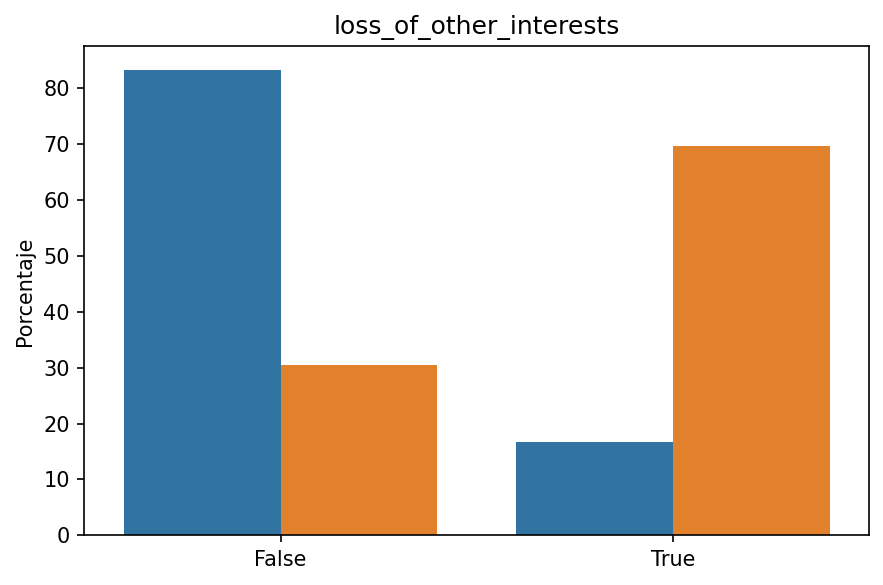
\includegraphics[width=\textwidth]{images/categoricas/loss_of_other_interests.png}
        \caption{Pérdida de otros intereses}
    \end{subfigure}
    \hfill
    \begin{subfigure}[b]{0.48\textwidth}
        \centering
        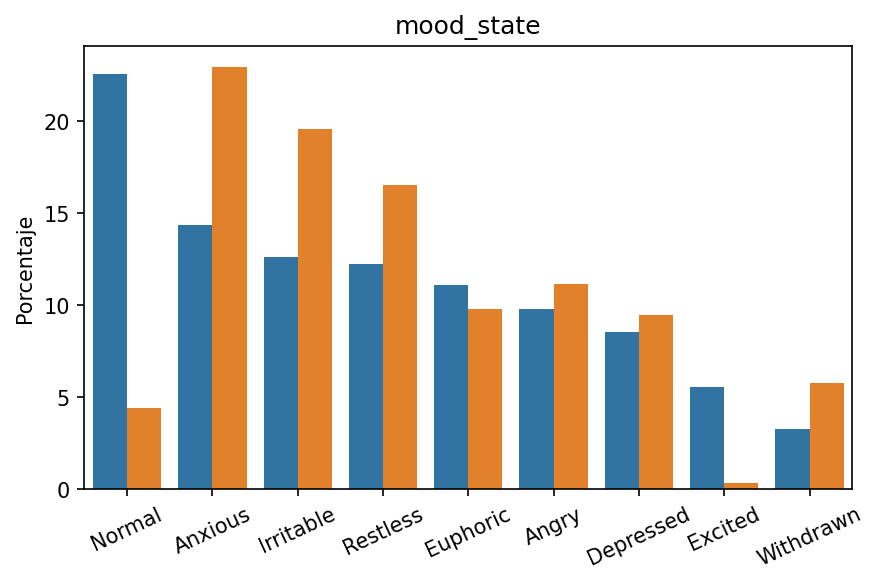
\includegraphics[width=\textwidth]{images/categoricas/mood_state.png}
        \caption{Estado de ánimo}
    \end{subfigure}
    \vspace{10pt}
    \begin{subfigure}[b]{0.48\textwidth}
        \centering
        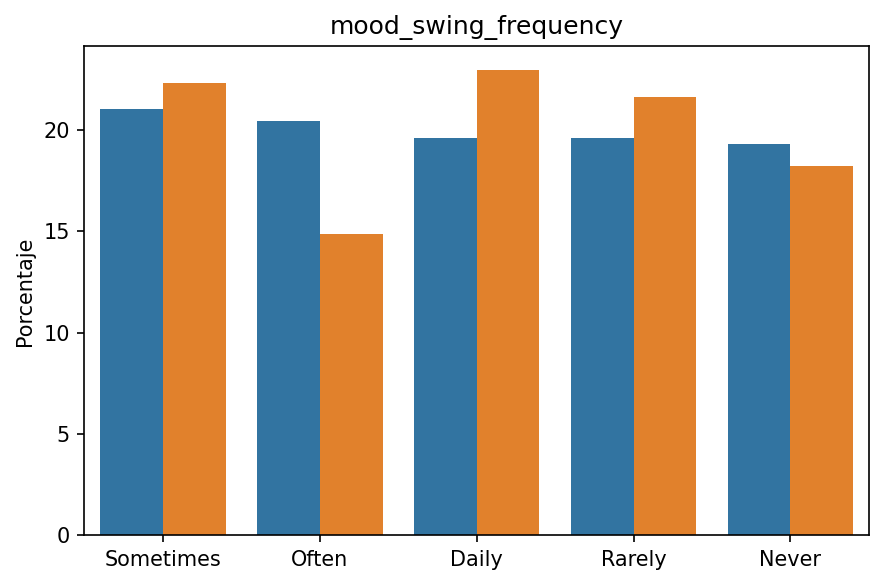
\includegraphics[width=\textwidth]{images/categoricas/mood_swing_frequency.png}
        \caption{Frecuencia de cambios de humor}
    \end{subfigure} 
    \hfill
    \begin{subfigure}[b]{0.48\textwidth}
        \centering
        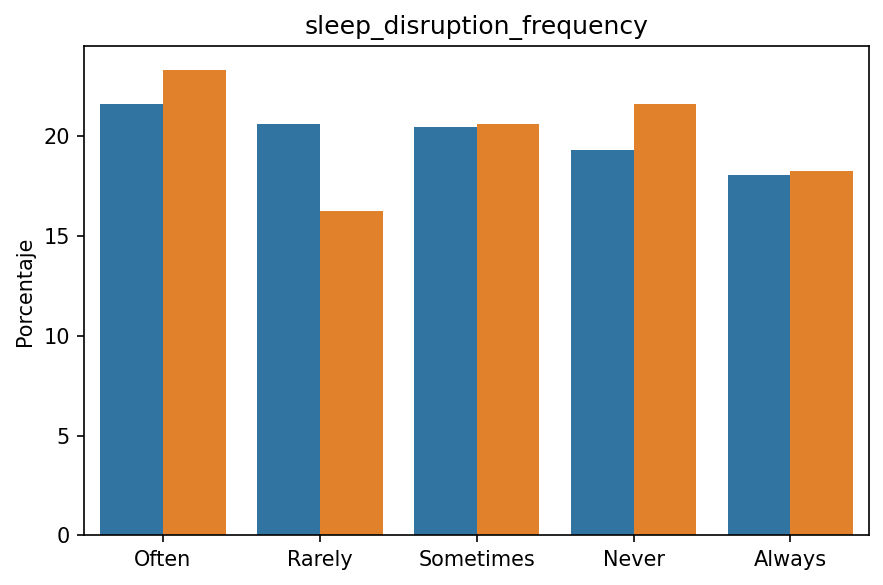
\includegraphics[width=\textwidth]{images/categoricas/sleep_disruption_frequency.png}
        \caption{Frecuencia de alteraciones del sueño}
    \end{subfigure}
    \vspace{10pt}
    \begin{subfigure}[b]{0.48\textwidth}
        \centering
        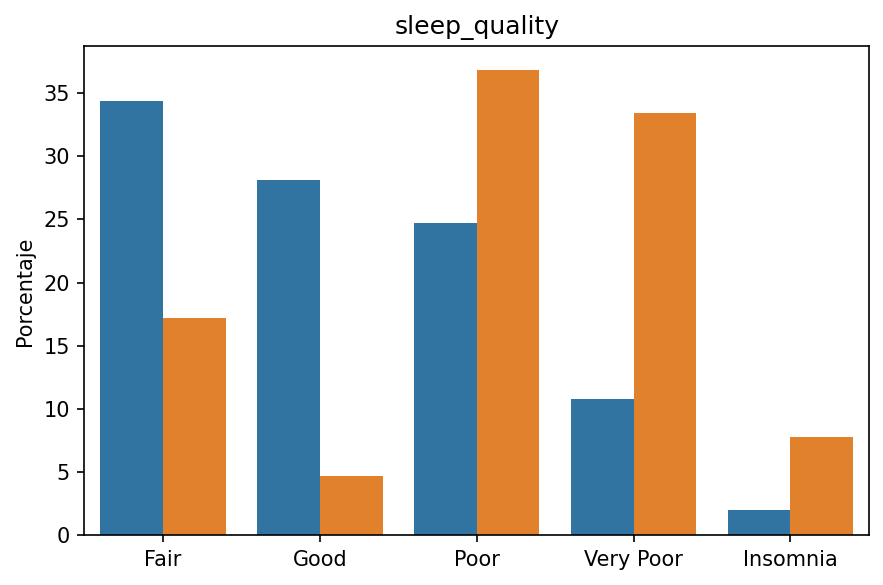
\includegraphics[width=\textwidth]{images/categoricas/sleep_quality.png}
        \caption{Calidad del sueño}
    \end{subfigure}
    \hfill
    \begin{subfigure}[b]{0.48\textwidth}
        \centering
        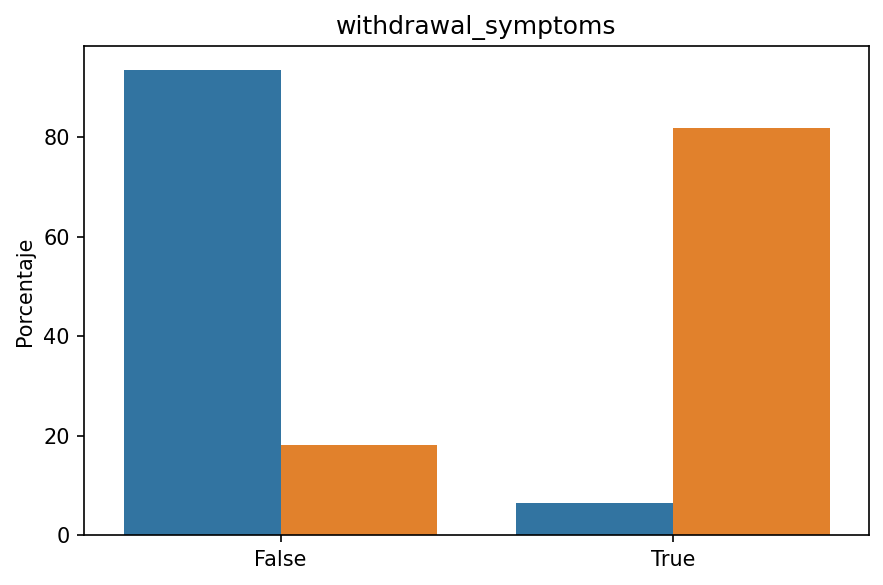
\includegraphics[width=\textwidth]{images/categoricas/withdrawal_symptoms.png}
        \caption{Síntomas de abstinencia}
    \end{subfigure}

    \caption{Diagramas de barras de cada variable categórica según la clase 
    (\textcolor[HTML]{3274a1}{$\blacksquare$} \textit{Low Risk}, \textcolor[HTML]{e0802c}{$\blacksquare$} \textit{High Risk})}
    \label{fig:analisis_categorico}
\end{figure}

Se puede observar como hay variables donde el porcentaje de ejemplos dentro de ambas clases es similar, como \textit{game\_genre} o \textit{gender}, por lo que no parecen aportar demasiada información que pueda diferenciar a ambos grupos. 

En general, las variables categóricas de verdadero o falso muestran una clara diferencia entre clases. Sintomas físicos, como el dolor de espalda/cuello o la fatiga visual son más propios de personas con riesgo de adicción a los videojuegos, por su habitual mala postura y sus largas sesiones de juego. 
En cuanto a los síntomas psicológicos, parece lógico pensar que las personas que continúan jugando a pesar de los problemas presentes en sus vidas tienen más riesgo de sufrir una adicción a los videojuegos. La pérdida de otros intereses puede deberse a una adicción... % cambiar esto último, no se 

comentar algo de lo de la abstinencia

El género del videojuego no parece agravar el riesgo de adicción, salvo si es \textit{MOBA}, \textit{RPG}, \textit{FPS} o \textit{Battle Royale}.

comentar algo mas


\subsubsection{Variables categóricas (probabilidad de \textit{High Risk})} 
Como el objetivo es poder clasificar correctamente a individuos que tengan un riesgo alto de caer en una adicción a los videojuegos, en las siguientes gráficas se muestra la probabilidad de que un ejemplo sea clasificado como de alto riesgo (que sea de la clase positiva) según su categoría para cada variable categórica.\newline

La línea roja discontinua representa la probabilidad a priori de que un individuo sea de alto riesgo ($P(High Risk) = 0.3$). Así se puede observar si determinadas categorías presentan un riesgo superior al promedio. 

\begin{figure}[H]
    \centering
    \begin{subfigure}[b]{0.45\textwidth}
        \centering
        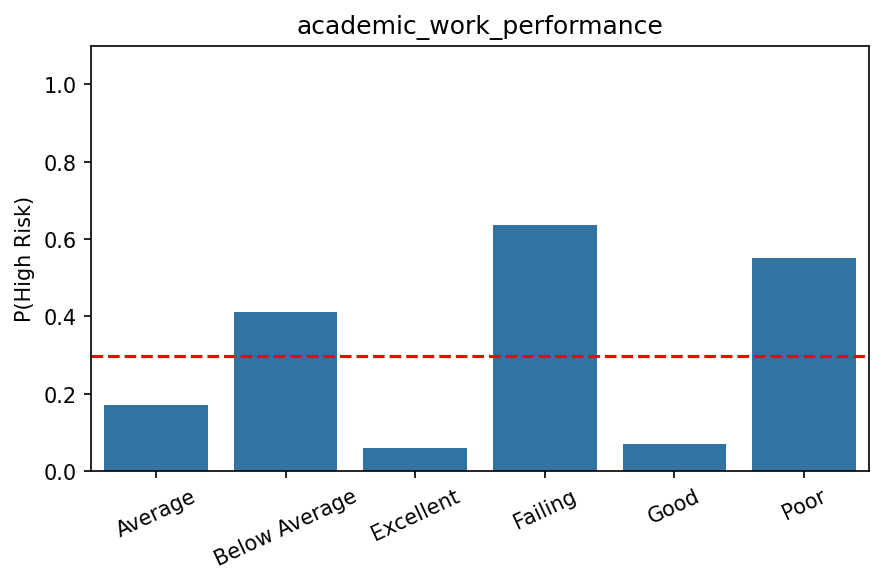
\includegraphics[width=\textwidth]{images/categoricas_alternativa/academic_work_performance_alt.png}
        \caption{Rendimiento académico/laboral}
    \end{subfigure}
    \hfill
    \begin{subfigure}[b]{0.45\textwidth}
        \centering
        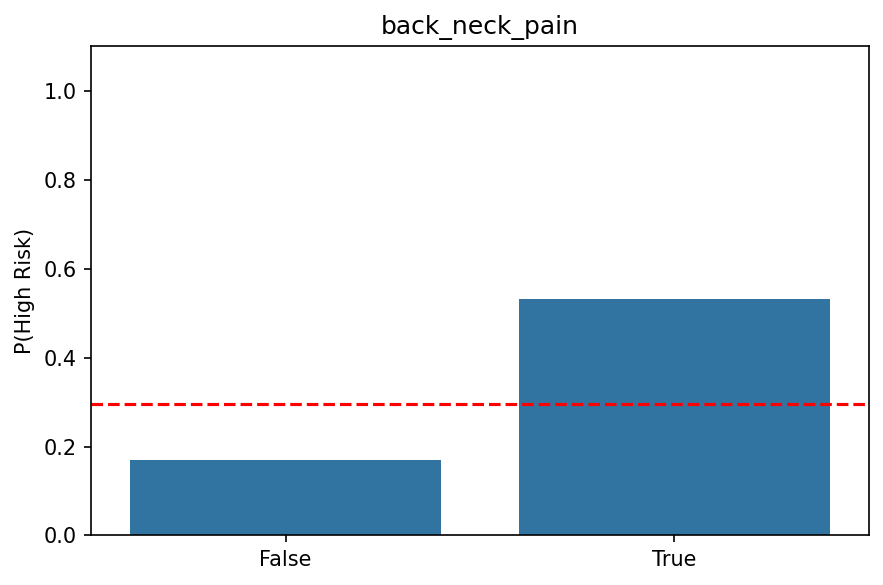
\includegraphics[width=\textwidth]{images/categoricas_alternativa/back_neck_pain_alt.png}
        \caption{Dolor de espalda/cuello}
    \end{subfigure}
    \begin{subfigure}[b]{0.45\textwidth}
        \centering
        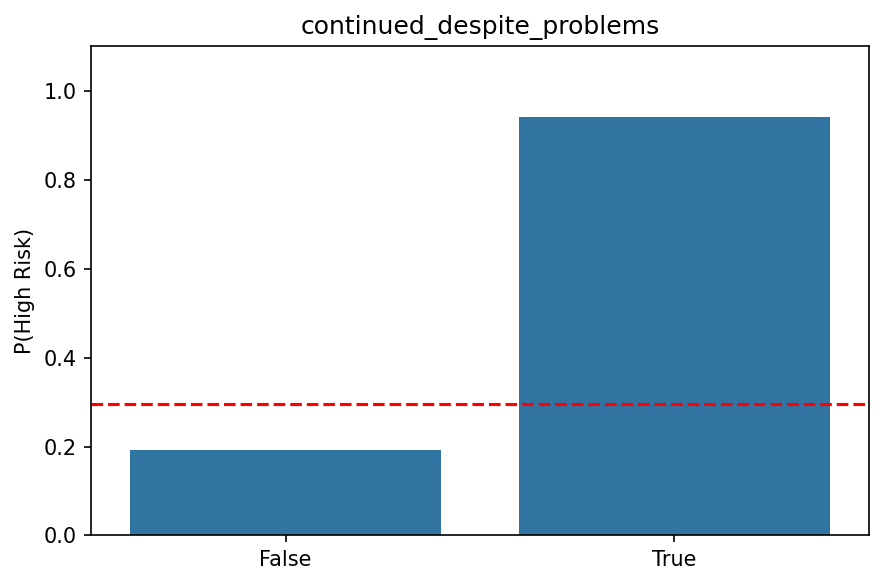
\includegraphics[width=\textwidth]{images/categoricas_alternativa/continued_despite_problems_alt.png}
        \caption{Continúa jugando a pesar de los problemas}
    \end{subfigure}
    \hfill
    \begin{subfigure}[b]{0.45\textwidth}
        \centering
        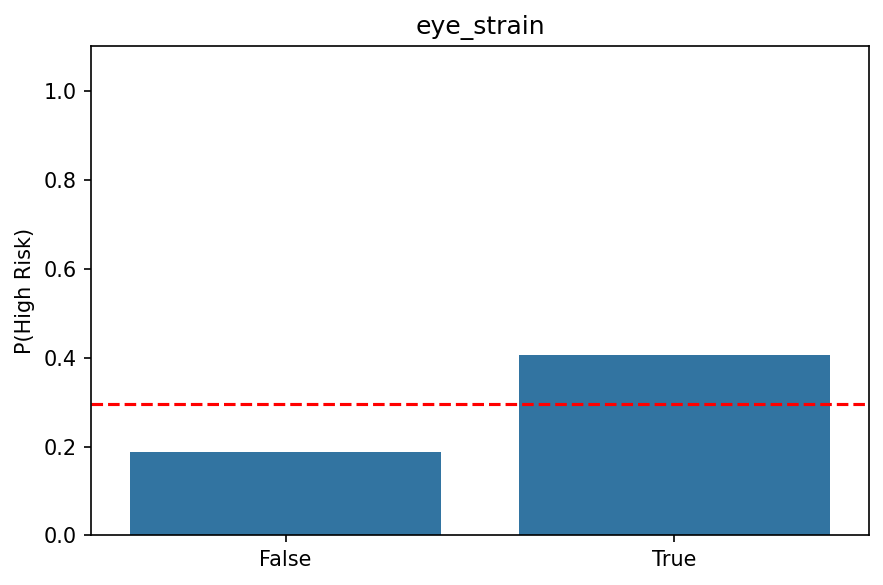
\includegraphics[width=\textwidth]{images/categoricas_alternativa/eye_strain_alt.png}
        \caption{Fatiga visual}
    \end{subfigure}
\end{figure}
\begin{figure}[H]
    \centering
    \ContinuedFloat
    \begin{subfigure}[b]{0.45\textwidth}
        \centering
        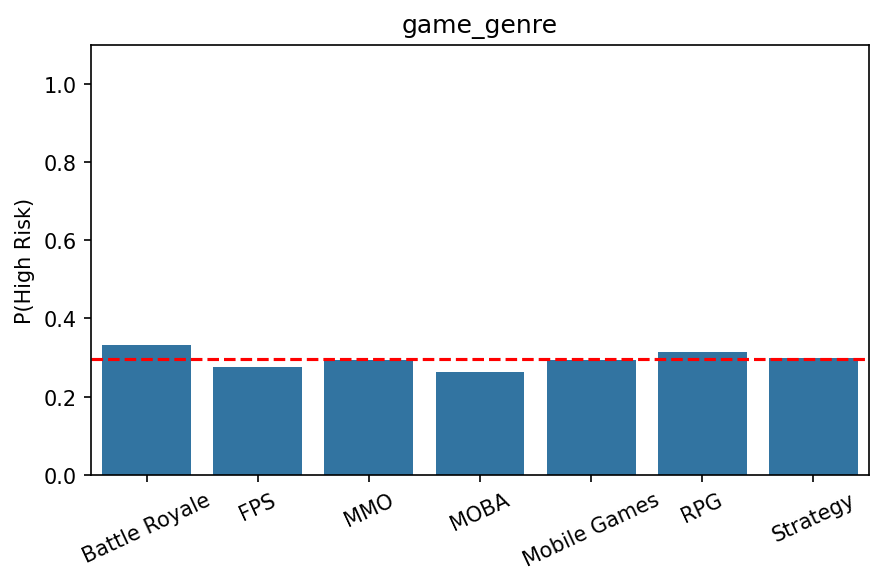
\includegraphics[width=\textwidth]{images/categoricas_alternativa/game_genre_alt.png}
        \caption{Género de videojuego}
    \end{subfigure}
    \hfill
    \begin{subfigure}[b]{0.45\textwidth}
        \centering
        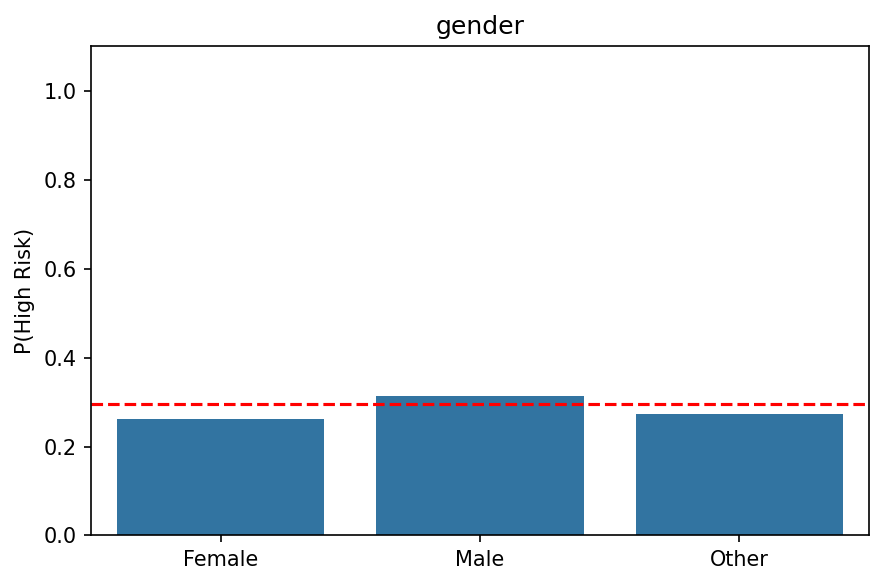
\includegraphics[width=\textwidth]{images/categoricas_alternativa/gender_alt.png}
        \caption{Género}
    \end{subfigure}
    \begin{subfigure}[b]{0.45\textwidth}
        \centering
        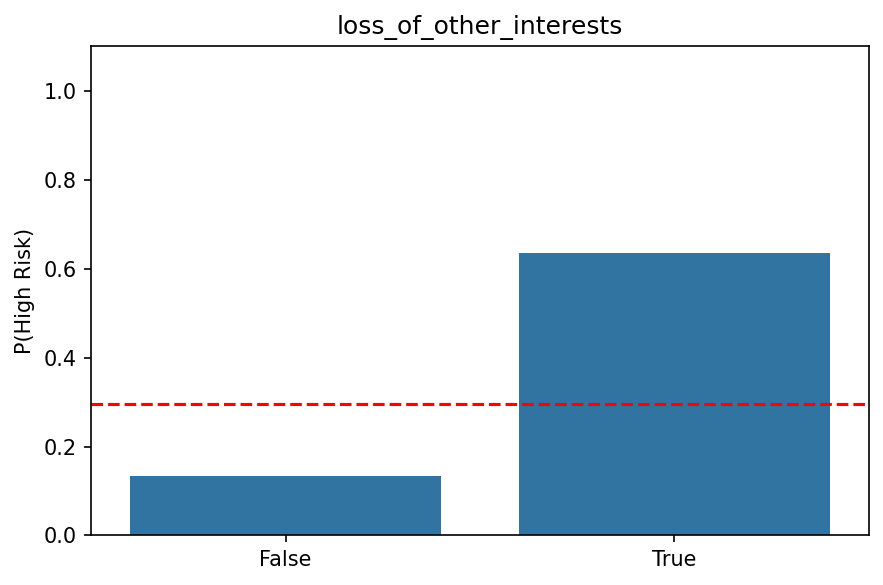
\includegraphics[width=\textwidth]{images/categoricas_alternativa/loss_of_other_interests_alt.png}
        \caption{Pérdida de otros intereses}
    \end{subfigure}
    \hfill
    \begin{subfigure}[b]{0.45\textwidth}
        \centering
        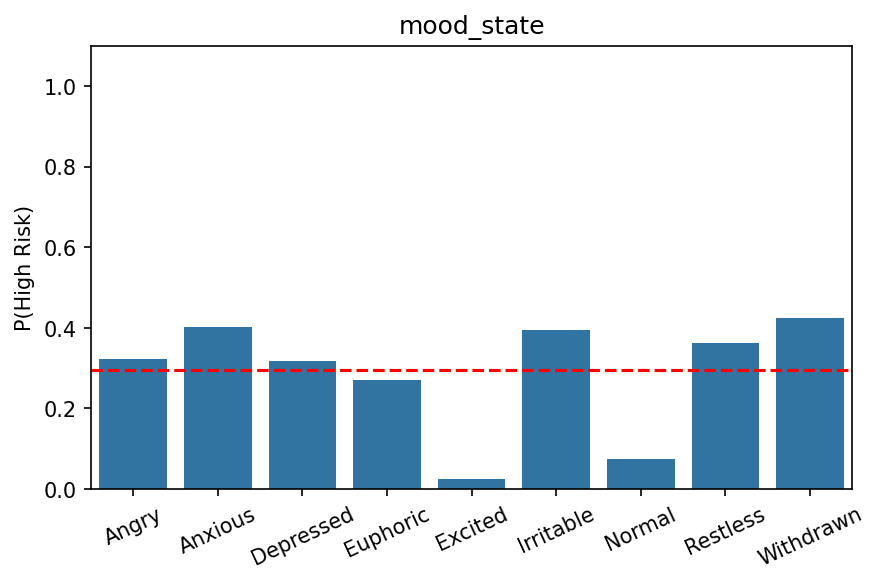
\includegraphics[width=\textwidth]{images/categoricas_alternativa/mood_state_alt.png}
        \caption{Estado de ánimo}
    \end{subfigure}
    \begin{subfigure}[b]{0.45\textwidth}
        \centering
        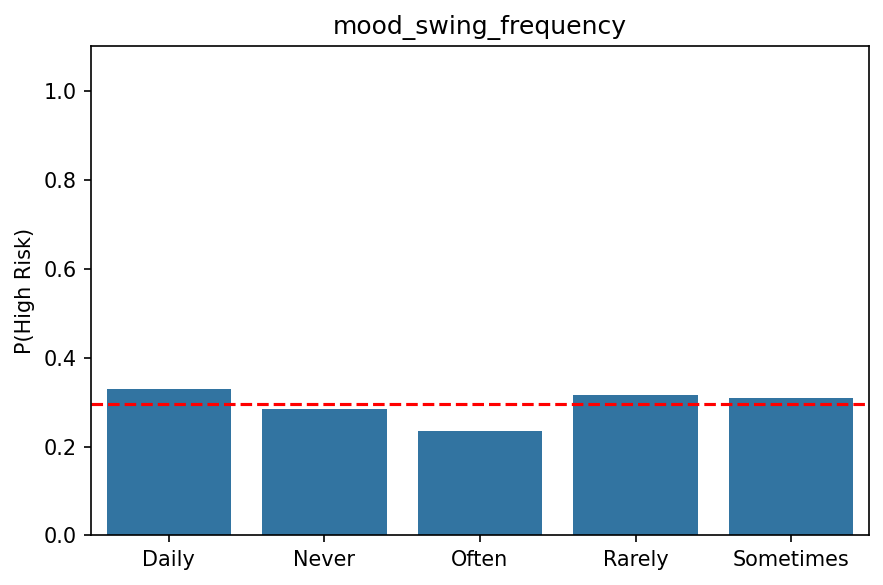
\includegraphics[width=\textwidth]{images/categoricas_alternativa/mood_swing_frequency_alt.png}
        \caption{Frecuencia de cambios de humor}
    \end{subfigure}
    \hfill
    \begin{subfigure}[b]{0.45\textwidth}
        \centering
        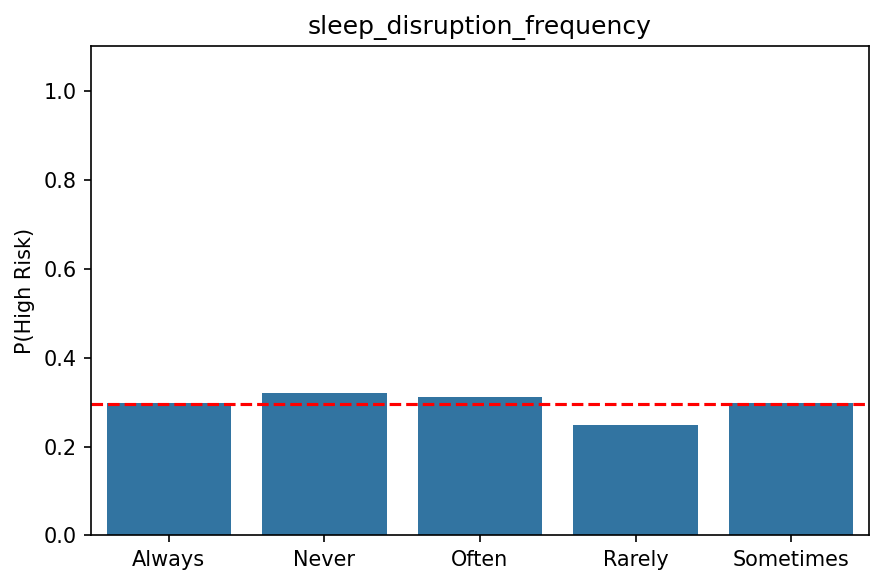
\includegraphics[width=\textwidth]{images/categoricas_alternativa/sleep_disruption_frequency_alt.png}
        \caption{Frecuencia de alteraciones del sueño}
    \end{subfigure}
\end{figure}
\begin{figure}[H]
    \centering
    \ContinuedFloat
    \begin{subfigure}[b]{0.45\textwidth}
        \centering
        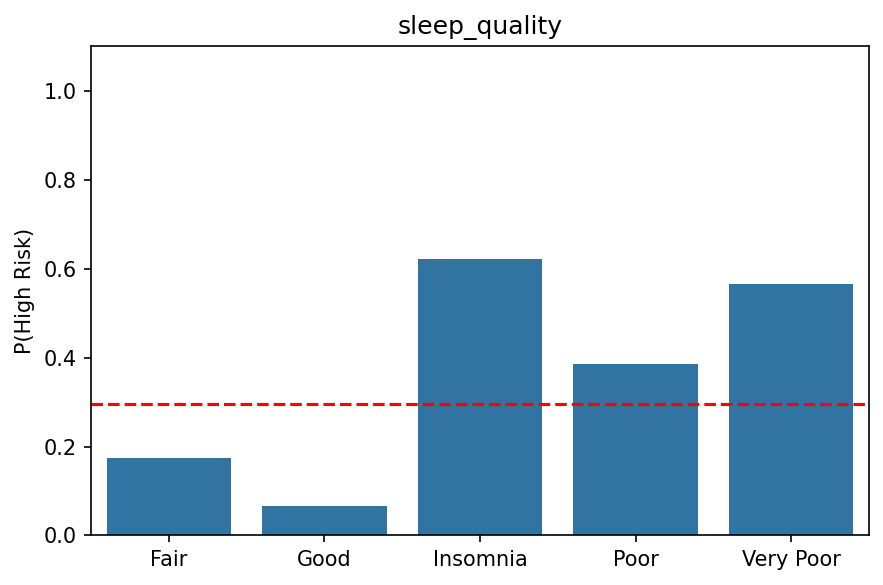
\includegraphics[width=\textwidth]{images/categoricas_alternativa/sleep_quality_alt.png}
        \caption{Calidad del sueño}
    \end{subfigure}
    \hfill
    \begin{subfigure}[b]{0.45\textwidth}
        \centering
        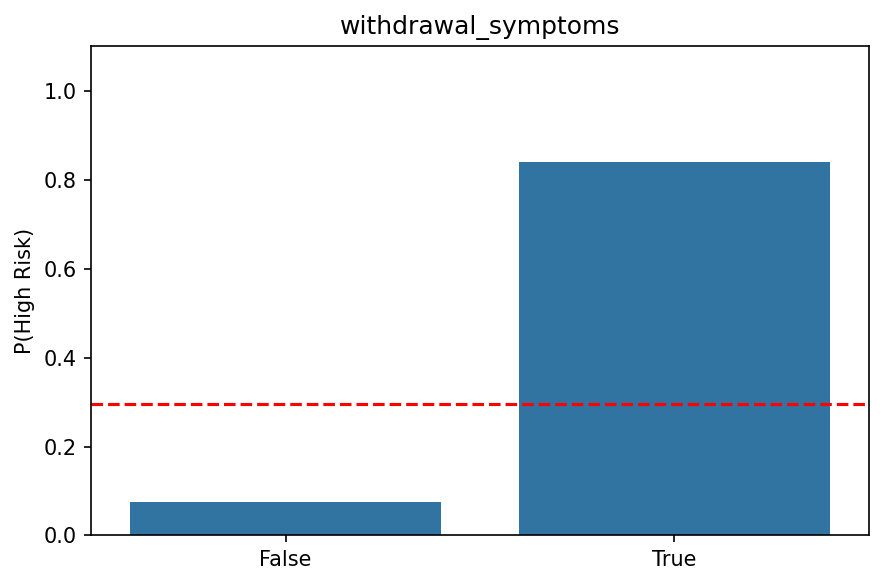
\includegraphics[width=\textwidth]{images/categoricas_alternativa/withdrawal_symptoms_alt.png}
        \caption{Síntomas de abstinencia}
    \end{subfigure}

    \caption{Probabilidad de \textit{High Risk} por categoría en cada variable categórica.} 
    \label{fig:analisis_categorico_alt}
\end{figure}


\section{Rendimiento y validación}

Ante un problema, antes de construir una solución se debe planificar bien cómo se va a medir la calidad de un modelo, definiendo las métricas de rendimiento empleadas, así como la metodología de validación a emplear.

\subsection{Métricas de rendimiento}

En el caso de este proyecto, se trata de un problema de clasificación en el que se predice el nivel de riesgo de adicción a los videojuegos de una persona: alto o bajo. Por lo tanto, se tratará de minimizar el número de personas con riesgo de adicción alto clasificadas erróneamente (falsos negativos). Se ha llegado a esta conclusión considerando que las consecuencias que supondría un error de este tipo son más dañinas que las que supondría cometer el error inverso: clasificar a una persona con riesgo de adicción bajo erróneamente (falsos positivos).\newline

Debido a lo anterior, como métrica independiente del umbral se ha escogido el \textbf{área bajo la curva Precision-Recall (PR)}, que resulta especialmente útil en problemas en los que se debe clasificar bien una clase (en este caso, las personas con riesgo alto).\newline

Por otro lado, como métrica dependiente del umbral se ha elegido el \textit{\textbf{f1-score}} porque, al tener en cuenta tanto la \textit{precisión} como el \textit{recall}, consigue llegar a un balance entre detectar una proporción razonable de casos positivos y evitar los falsos positivos que pueden acarrear preocupaciones innecesarias.

\subsection{Metodología de validación}

La metodología de validación empleada en el proyecto ha sido \textbf{validación cruzada}, con $k = 5$. Se ha escogido esta porque, al tratarse de un dataset no muy extenso (unos 1000 ejemplos), las mejoras que introduce respecto al hold out (se emplean todos los ejemplos para entrenar y validar el modelo) compensan el aumento del coste computacional.\newline

Para escoger el mejor modelo de entre un conjunto de pipelines, se itera sobre cada una de las opciones y se realiza el proceso de validación, empleando el área bajo la curva Precision-Recall como métrica. Una vez se escoge el mejor modelo con la métrica independiente del umbral, se emplea de nuevo el conjunto de validación pero, esta vez, con el fin de encontrar el mejor umbral para el f1-score. Finalmente, con el mejor modelo y el mejor umbral, se calcula el rendimiento en el conjunto de test.\newline

diagrama del proceso?

\section{Experimentos realizados}

Una vez definidas las métricas de rendimiento y la metodología de validación a emplear, es posible experimentar con diferentes técnicas
de preprocesamiento de datos para averiguar cuáles son las que obtienen mejores resultados y por qué (no me convence el 'y por qué').

\subsection{Fases del preprocesamiento}

Existen diferentes fases de preprocesamiento que se pueden aplicar a los datos antes de entrenar un modelo de clasificación. En este
proyecto, la organización de las fases se ha dispuesto de la siguiente manera:

\begin{figure}[H]
    \centering
    \ttfamily
    \fbox{División del dataset} 

    \vspace{0.2cm}$\downarrow$ \vspace{0.2cm}
    
    \fbox{Imputación de valores perdidos} $\rightarrow$ \fbox{Transformación de tipos} $\rightarrow$
    
    \vspace{0.5cm}

    \fbox{Detección de Outliers} $\rightarrow$ \fbox{Estandarización} $\rightarrow$
    
    \vspace{0.5cm}
    
    \fbox{Generación/Transformación de variables} $\rightarrow$ \fbox{Selección de variables} $\rightarrow$

    \vspace{0.2cm}$\downarrow$ \vspace{0.2cm}

    \fbox{\textbf{Clasificador}}
    
    \caption{Diagrama del flujo de los datos a través de los componentes del modelo.}
\end{figure}

\subsection{Técnicas para cada fase}

Con el fin de obtener un modelo robusto, se han implementado diferentes técnicas de preprocesamiento de datos para cada fase de la
pipeline, de las cuales se escogerán las mejores resultados obtengan. \newline

comentar que se eligen secuencialmente no todas a la vez, eso es debido a la alta combinatoria... blablabla hay que decir en algun momento que el clasificador empleado es KNN no se dice hasta ahora CREO !!!!!!

\subsubsection{Imputación de valores perdidos}

Tras analizar la presencia de valores perdidos en el dataset, se encontró que faltaban valores para las variables \textit{grades\_gpa} y
\textit{work\_productivity\_score}. Al ser ambas variables numéricas, se ha escogido una serie de métodos de imputación posibles:

\begin{itemize}
    \item Imputación por el vecino más cercano
    \item Imputación por la media
    \item Imputación por la mediana
\end{itemize}

\subsubsection{Transformación de tipos}

Tras imputar los valores faltantes, es necesaria una transformación del tipo de los datos: las variables categóricas deben ser transformadas
al espacio numérico. Esto es debido a la naturaleza del modelo de clasificación, ya que KNN se basa en la \textit{distancia}
entre los valores de las variables para determinar sus resultados. \newline

Sin embargo, no todas las variables categóricas se deben transformar de la misma manera. Existen variables cuyos valores tienen un orden,
variables booleanas y variables sin orden. En cada caso, se aplica una transformación diferente. Para las variables cuyas categorías siguen un orden, como en el caso de \textit{sleep\_quality}: \{..., Poor, Fair, Good, ...\}, se emplea la codificación ordinal. Para variables booleanas, se transforma el valor True en 1 y el valor False en 0. \newline

Sin embargo, para las variables sin orden con varias categorías existen múltiples opciones válidas. En este caso, se han
escogido los siguientes métodos de codificación:

\begin{itemize}
    \item Codificación binaria
    \item Codificación basada en la salida
\end{itemize}

\subsubsection{Detección de outliers}

Una vez los datos son transformados a formato numérico, resulta natural aplicar un proceso de detección de outliers, sobre
todo antes de la fase de estandarización, donde los ejemplos atípicos pueden tener mucha influencia según el método escogido. (no me acaba de convencer, molaria justificarlo algo más) \newline

Los métodos de detección de outliers empleados son:

\begin{itemize}
    \item Método de la media-desviación
    \item Método del rango intercuartil (IQR)
\end{itemize}

Cada método se probará con diferentes valores de $k \in \{1.5, 2, 2.5, 3\}$ y, en caso de detectar un valor atípico, lo sustituirá por la mediana de los datos de entrenamiento.

\subsubsection{Estandarización}

Tras detectar y corregir los outliers presentes en el dataset, es posible realizar una normalización de los datos para
que todas las variables se encuentren en un rango similar. Esto es positivo porque, empleando KNN como método de clasificación (o cualquier método basado en distancias), las variables con rango más amplio tendrán una mayor importancia
a la hora de clasificar instancias. (epxlicar mejro estoy 0 inspirado a las 9pm)\newline

Los posibles métodos de estandarización son:

\begin{itemize}
    \item Estandarización Min-Max
    \item Estandarización z-score
    \item Método Robust-scaler
\end{itemize}

\subsubsection{Generación y transformación de variables}

\subsubsection{Selección de variables}

\section{Resultados}

explicar resultados, graficas, interpretabilidad del modelo


\section{Conclusiones}

explicar conclusiones


\end{document}